% Options for packages loaded elsewhere
\PassOptionsToPackage{unicode}{hyperref}
\PassOptionsToPackage{hyphens}{url}
%
\documentclass[
]{article}
\usepackage{amsmath,amssymb}
\usepackage{lmodern}
\usepackage{ifxetex,ifluatex}
\ifnum 0\ifxetex 1\fi\ifluatex 1\fi=0 % if pdftex
  \usepackage[T1]{fontenc}
  \usepackage[utf8]{inputenc}
  \usepackage{textcomp} % provide euro and other symbols
\else % if luatex or xetex
  \usepackage{unicode-math}
  \defaultfontfeatures{Scale=MatchLowercase}
  \defaultfontfeatures[\rmfamily]{Ligatures=TeX,Scale=1}
\fi
% Use upquote if available, for straight quotes in verbatim environments
\IfFileExists{upquote.sty}{\usepackage{upquote}}{}
\IfFileExists{microtype.sty}{% use microtype if available
  \usepackage[]{microtype}
  \UseMicrotypeSet[protrusion]{basicmath} % disable protrusion for tt fonts
}{}
\makeatletter
\@ifundefined{KOMAClassName}{% if non-KOMA class
  \IfFileExists{parskip.sty}{%
    \usepackage{parskip}
  }{% else
    \setlength{\parindent}{0pt}
    \setlength{\parskip}{6pt plus 2pt minus 1pt}}
}{% if KOMA class
  \KOMAoptions{parskip=half}}
\makeatother
\usepackage{xcolor}
\IfFileExists{xurl.sty}{\usepackage{xurl}}{} % add URL line breaks if available
\IfFileExists{bookmark.sty}{\usepackage{bookmark}}{\usepackage{hyperref}}
\hypersetup{
  pdftitle={A Guide to Mapping ICPSR Data in R Studio},
  pdfauthor={Aditya Ranganath},
  hidelinks,
  pdfcreator={LaTeX via pandoc}}
\urlstyle{same} % disable monospaced font for URLs
\usepackage[margin=1in]{geometry}
\usepackage{color}
\usepackage{fancyvrb}
\newcommand{\VerbBar}{|}
\newcommand{\VERB}{\Verb[commandchars=\\\{\}]}
\DefineVerbatimEnvironment{Highlighting}{Verbatim}{commandchars=\\\{\}}
% Add ',fontsize=\small' for more characters per line
\usepackage{framed}
\definecolor{shadecolor}{RGB}{248,248,248}
\newenvironment{Shaded}{\begin{snugshade}}{\end{snugshade}}
\newcommand{\AlertTok}[1]{\textcolor[rgb]{0.94,0.16,0.16}{#1}}
\newcommand{\AnnotationTok}[1]{\textcolor[rgb]{0.56,0.35,0.01}{\textbf{\textit{#1}}}}
\newcommand{\AttributeTok}[1]{\textcolor[rgb]{0.77,0.63,0.00}{#1}}
\newcommand{\BaseNTok}[1]{\textcolor[rgb]{0.00,0.00,0.81}{#1}}
\newcommand{\BuiltInTok}[1]{#1}
\newcommand{\CharTok}[1]{\textcolor[rgb]{0.31,0.60,0.02}{#1}}
\newcommand{\CommentTok}[1]{\textcolor[rgb]{0.56,0.35,0.01}{\textit{#1}}}
\newcommand{\CommentVarTok}[1]{\textcolor[rgb]{0.56,0.35,0.01}{\textbf{\textit{#1}}}}
\newcommand{\ConstantTok}[1]{\textcolor[rgb]{0.00,0.00,0.00}{#1}}
\newcommand{\ControlFlowTok}[1]{\textcolor[rgb]{0.13,0.29,0.53}{\textbf{#1}}}
\newcommand{\DataTypeTok}[1]{\textcolor[rgb]{0.13,0.29,0.53}{#1}}
\newcommand{\DecValTok}[1]{\textcolor[rgb]{0.00,0.00,0.81}{#1}}
\newcommand{\DocumentationTok}[1]{\textcolor[rgb]{0.56,0.35,0.01}{\textbf{\textit{#1}}}}
\newcommand{\ErrorTok}[1]{\textcolor[rgb]{0.64,0.00,0.00}{\textbf{#1}}}
\newcommand{\ExtensionTok}[1]{#1}
\newcommand{\FloatTok}[1]{\textcolor[rgb]{0.00,0.00,0.81}{#1}}
\newcommand{\FunctionTok}[1]{\textcolor[rgb]{0.00,0.00,0.00}{#1}}
\newcommand{\ImportTok}[1]{#1}
\newcommand{\InformationTok}[1]{\textcolor[rgb]{0.56,0.35,0.01}{\textbf{\textit{#1}}}}
\newcommand{\KeywordTok}[1]{\textcolor[rgb]{0.13,0.29,0.53}{\textbf{#1}}}
\newcommand{\NormalTok}[1]{#1}
\newcommand{\OperatorTok}[1]{\textcolor[rgb]{0.81,0.36,0.00}{\textbf{#1}}}
\newcommand{\OtherTok}[1]{\textcolor[rgb]{0.56,0.35,0.01}{#1}}
\newcommand{\PreprocessorTok}[1]{\textcolor[rgb]{0.56,0.35,0.01}{\textit{#1}}}
\newcommand{\RegionMarkerTok}[1]{#1}
\newcommand{\SpecialCharTok}[1]{\textcolor[rgb]{0.00,0.00,0.00}{#1}}
\newcommand{\SpecialStringTok}[1]{\textcolor[rgb]{0.31,0.60,0.02}{#1}}
\newcommand{\StringTok}[1]{\textcolor[rgb]{0.31,0.60,0.02}{#1}}
\newcommand{\VariableTok}[1]{\textcolor[rgb]{0.00,0.00,0.00}{#1}}
\newcommand{\VerbatimStringTok}[1]{\textcolor[rgb]{0.31,0.60,0.02}{#1}}
\newcommand{\WarningTok}[1]{\textcolor[rgb]{0.56,0.35,0.01}{\textbf{\textit{#1}}}}
\usepackage{longtable,booktabs,array}
\usepackage{calc} % for calculating minipage widths
% Correct order of tables after \paragraph or \subparagraph
\usepackage{etoolbox}
\makeatletter
\patchcmd\longtable{\par}{\if@noskipsec\mbox{}\fi\par}{}{}
\makeatother
% Allow footnotes in longtable head/foot
\IfFileExists{footnotehyper.sty}{\usepackage{footnotehyper}}{\usepackage{footnote}}
\makesavenoteenv{longtable}
\usepackage{graphicx}
\makeatletter
\def\maxwidth{\ifdim\Gin@nat@width>\linewidth\linewidth\else\Gin@nat@width\fi}
\def\maxheight{\ifdim\Gin@nat@height>\textheight\textheight\else\Gin@nat@height\fi}
\makeatother
% Scale images if necessary, so that they will not overflow the page
% margins by default, and it is still possible to overwrite the defaults
% using explicit options in \includegraphics[width, height, ...]{}
\setkeys{Gin}{width=\maxwidth,height=\maxheight,keepaspectratio}
% Set default figure placement to htbp
\makeatletter
\def\fps@figure{htbp}
\makeatother
\setlength{\emergencystretch}{3em} % prevent overfull lines
\providecommand{\tightlist}{%
  \setlength{\itemsep}{0pt}\setlength{\parskip}{0pt}}
\setcounter{secnumdepth}{5}
\ifluatex
  \usepackage{selnolig}  % disable illegal ligatures
\fi

\title{A Guide to Mapping ICPSR Data in R Studio}
\author{Aditya Ranganath}
\date{2021-09-21}

\begin{document}
\maketitle

{
\setcounter{tocdepth}{2}
\tableofcontents
}
\hypertarget{preface}{%
\section{Preface}\label{preface}}

This brief guide to mapping ICPSR data in R Studio was prepared as part of Aditya Ranganath's ICPSR Visiting Representative Fellowship in the summer and fall of 2021. It can be used as a lesson plan for instructors, as well as a tool for self-study.

\hypertarget{introduction}{%
\section{Introduction}\label{introduction}}

\hypertarget{motivation}{%
\subsection{Motivation}\label{motivation}}

Many of ICSPR's datasets are available in tabular formats that are ready to be imported into standard statistical software packages for analysis. In many cases, it is possible to visualize the data in these tabular datasets on a map (even if such visualizations are not explicitly a part of the original analysis or the replication materials provided by ICPSR). In this tutorial, we will provide a brief example-driven overview of how you can visually represent tabular information from an ICSPR dataset on a map, using packages written for the R programming language. The tutorial does not presuppose any previous experience with statistical analysis or programming.

Why map ICPSR data to begin with? Students and researchers often use data archived at ICPSR as a resource for exploration and discovery. Indeed, the data that others have collected can often inspire novel questions and hypotheses. It is also the case that the social and political processes studied by the researchers who archive their data with ICPSR are intrinsically spatial; after all, these processes necessarily occur somewhere on the surface of the earth! Placing these social and political processes in their spatial context can therefore bring the data encoded in tabular datasets to life in dramatic ways, helping us to quickly notice patterns, identify puzzles, and generate hypotheses that would have otherwise remained obscure. In addition to using ICPSR data to generate ideas and explore patterns in existing data, students and researchers may want to reuse ICPSR data and incorporate them into their own ongoing research projects; in reusing this data, they may find it helpful to make publishable maps that they can use in their own papers and projects.

\hypertarget{scope-and-objectives}{%
\subsection{Scope and Objectives}\label{scope-and-objectives}}

By working through the following code, students and researchers will learn how to spatially visualize existing ICPSR data to aid their exploration of datasets of interest, as well as create publishable maps that can be used in their papers and projects. The tutorial can be used as a self-study resource, as well as the basis for a classroom demonstration or activity.

It is important to emphasize that this is not a tutorial on Geographic Information Systems (GIS) writ large, and we do not cover important GIS concepts such as map projections and coordinate reference systems. If you use advanced mapping and spatial analysis in your work, you should learn these technical foundations (which are beyond the scope of our lesson here). It is also not a tutorial on the principles of cartography, which is a complex art and science that is also beyond our scope; however, it will show you how to customize maps in R, and you can use these skills (after reading up on cartography on your own) to make maps that conform to sound cartographic design principles. Our goal here is to make a functional and informative map, not a work of art.

\hypertarget{preliminaries-and-set-up}{%
\section{Preliminaries and Set-Up}\label{preliminaries-and-set-up}}

\hypertarget{data}{%
\subsection{Data}\label{data}}

The ICPSR data we will be mapping in this tutorial comes from a dataset archived on \href{https://www.openicpsr.org/openicpsr/}{OPENICPSR}. In particular, the dataset we will be using is entitled ``Governments' Responses to COVID-19'', which was collected by Simon Porcher, a researcher at the University of Paris. The dataset can be found \href{https://www.openicpsr.org/openicpsr/project/119061/version/V6/view}{here}, and the full citation information is below:

Porcher, Simon. Governments' Responses to COVID-19 (Response2covid19). Ann Arbor, MI: Inter-university Consortium for Political and Social Research {[}distributor{]}, 2020-11-08. \url{https://doi.org/10.3886/E119061V6}.

This panel dataset provides information on public health and economic interventions initiated by national governments in response to the Covid-19 Pandemic. It provides data in monthly increments from January 2020 to October 2020 for most of the world's sovereign countries. One of the variables in the dataset is an index (computed based on other variables in the dataset), that reflects the extent of government economic interventions to provide their populations with material support during the most acute phase of the Covid-19 Pandemic. The tutorial will explore how to display this country-level data on economic responses to Covid-19 on a world map.

If you would like to follow along with the tutorial, please download the data above to your computer, and save it in a directory that is specifically dedicated to this tutorial.

\hypertarget{r-and-r-studio-installation}{%
\subsection{R and R Studio Installation}\label{r-and-r-studio-installation}}

If you haven't already, please go ahead and install R and R Studio. R and R Studio must be installed separately; you should install R first, and then R Studio. R is the bare-bones computing environment, while R Studio is a visually appealing and user-friendly interface that allows you to interact with this environment in an intuitive way. Once you have both installed, you don't need to open up R and R Studio separately; you only need to interact with R Studio (which will run R in the background).

The following subsections provide instructions on installing R and R Studio for the macOS and Windows operating systems. These instructions are taken from the ``Setup'' section of the Data Carpentry Course entitled \href{https://datacarpentry.org/r-socialsci/setup.html}{\emph{R for Social Scientists}}. The Data Carpentry page also contains installation instructions for the Linux operating system; if you're a Linux user, please refer to that page for instructions.

The Appendix to Garret Grolemund's book \emph{Hands on Programming with R} provides an excellent overview of the R and R Studio installation process; you can access it \href{https://rstudio-education.github.io/hopr/}{here}.

\hypertarget{windows-installation-instructions}{%
\subsubsection{Windows Installation Instructions}\label{windows-installation-instructions}}

\begin{itemize}
\tightlist
\item
  Download R from the \href{https://cran.r-project.org/bin/windows/base/}{CRAN website}
\item
  Run the \texttt{.exe} file that was just downloaded.
\item
  Go to the \href{https://www.rstudio.com/products/rstudio/download/\#download}{R Studio download page} and under \emph{Installers} select the ``Windows'' option.
\item
  Double click the file to install R Studio
\item
  Open R Studio to make sure it works.
\end{itemize}

\hypertarget{macos-installation-instructions}{%
\subsubsection{macOS Installation Instructions}\label{macos-installation-instructions}}

\begin{itemize}
\tightlist
\item
  Download R from the \href{https://cran.r-project.org/bin/macosx/}{CRAN website}
\item
  Select the \texttt{.pkg} file for the latest R version.
\item
  Double click on the downloaded file to install R.
\item
  It is also a good idea to install \href{https://www.xquartz.org/}{XQuartz}, which some packages require.
\item
  Go to the \href{https://www.rstudio.com/products/rstudio/download/\#download}{R Studio download page}, and under \emph{Installers} select the ``macOS'' option.
\item
  Double click the file to install R Studio
\item
  Open R Studio to make sure it works.
\end{itemize}

\hypertarget{the-r-studio-interface}{%
\subsection{The R Studio Interface}\label{the-r-studio-interface}}

Now that we've installed and opened up R Studio, let's familiarize ourselves with the R Studio interface. When you open up R Studio, you'll see a window open that looks something like this:

\begin{figure}
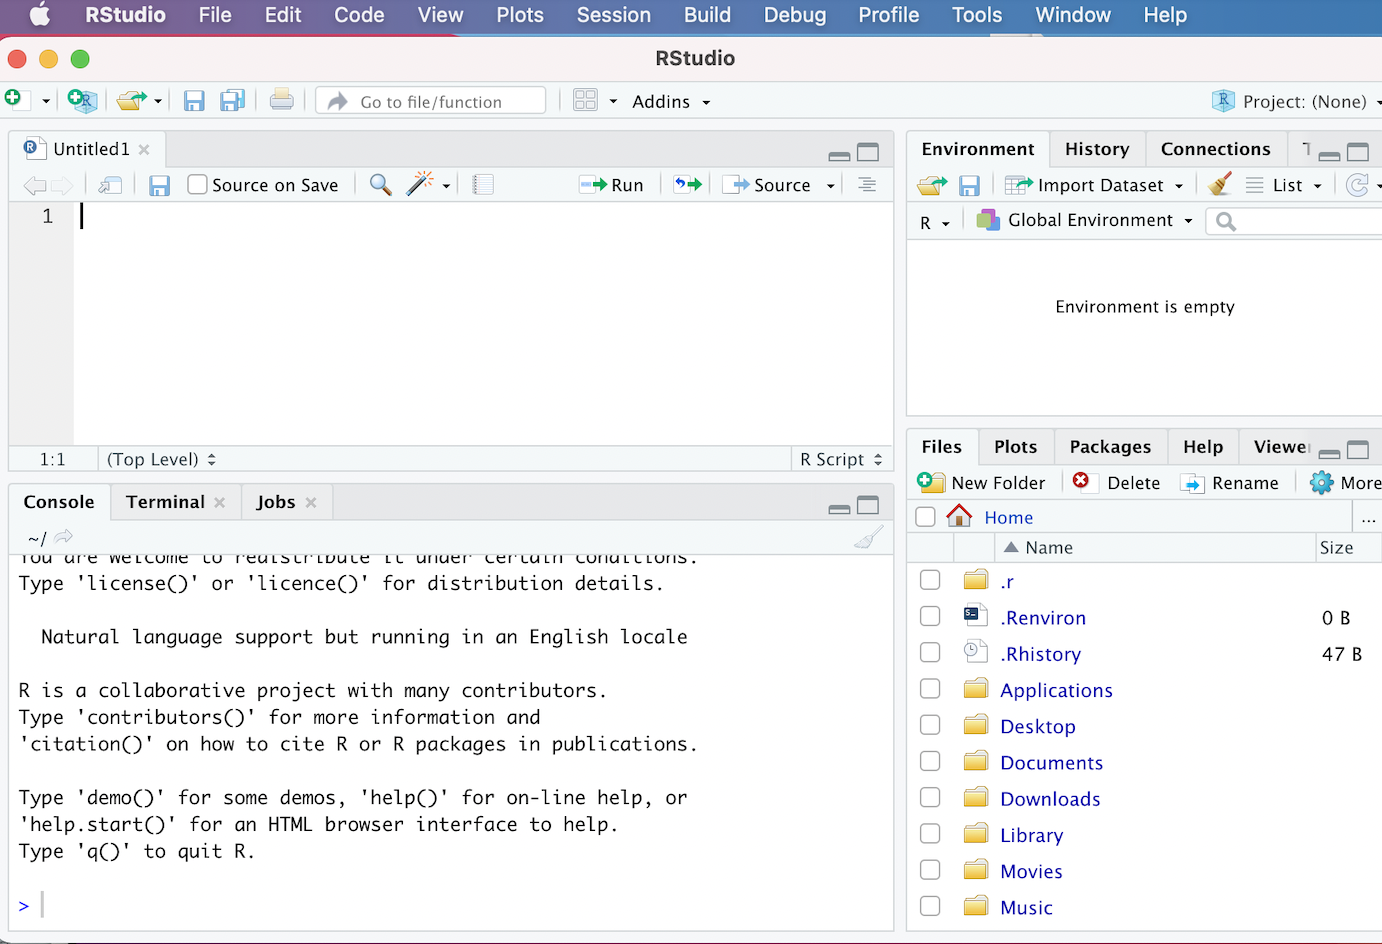
\includegraphics[width=1\linewidth]{images/rstudio_window_revised} \caption{The R Studio Interface}\label{fig:unnamed-chunk-1}
\end{figure}

If your interface doesn't look exactly like this, it shouldn't be a problem; we would expect to see minor cosmetic differences across operating systems and computers (based on how they're configured). However, you should see four distinct windows within the larger R Studio interface:

\begin{itemize}
\tightlist
\item
  The \textbf{top-left} window is known as the \emph{Source}.

  \begin{itemize}
  \tightlist
  \item
    The \emph{Source} window is where you can write your R scripts (including the code associated with this tutorial), and execute those scripts. You can also type in R code into the ``Console'' window (bottom-left window), but it is preferable to write your code in a script within the source window. That's because scripts can be saved (while code written into the console cannot); writing scripts therefore allows you to keep track of what you're doing, and facilitates the reproducibility of your work. Note that in some cases, you may not see a \emph{Source} window when you first open R Studio. In that case, to start a new script, simply click the \texttt{File} button on the R Studio menu bar, scroll down to \texttt{New\ File} button, and then select \texttt{R\ Script} from the menu bar that opens up.
  \item
    It's also worth noting that the outputs of certain functions will appear in the \emph{Source} window. In the context of our tutorial, when we want to view our tabular datasets or attribute tables (an attribute table is a table that provides information about the attributes of different geographic locations in a spatial dataset), we will use the \texttt{View()} function, which will display the relevant data within a new tab in the \emph{Source} window.
  \end{itemize}
\item
  The \textbf{top-right} window is the \emph{Environment/History} pane of the R Studio interface.

  \begin{itemize}
  \tightlist
  \item
    The ``Environment'' tab of this window provides information on the datasets you've loaded into R Studio, as well as objects you have defined (we'll talk about objects more later in the tutorial).
    -The ``History'' tab of the window provides a record of the R commands you've run in a given session.
  \end{itemize}
\item
  The \textbf{bottom-right} window is the \emph{Files/Plots/Packages/Help/Viewer} window.

  \begin{itemize}
  \tightlist
  \item
    The ``Files'' tab displays your computer's directories and file structures and allows you to navigate through them without having to leave the R environment.
    -The ``Plots'' tab is the tab where you can view any visualizations (including maps) that you create. Within the ``Plots'' tab, make note of the ``Zoom'' button, which you can use to enlarge your maps and visualizations if they're too compressed in the ``Plots'' window. Also, note the ``Export'' button within the ``Plots'' tab (next to the ``Zoom'' button); you can use this button to export the displayed map to a .png or .jpeg file that can be used outside of R Studio (you can also export your visualizations programmatically, which we'll cover how to do later in the tutorial).
  \item
    The ``Packages'' tab provides information on which packages have been installed, as well as which packages are currently loaded (more on packages in Section 3.4)
  \item
    The ``Help'' tab displays documentation for R packages and functions. If you want to know more about how a package or function work, simply type a ? followed by the package or function's name (no space between the question mark and the name) and relevant information will be displayed within the ``Help'' tab.
  \item
    The ``Viewer'' tab displays HTML output. If you write code that generates an HTML file, you can view it within the ``Viewer'' tab.
  \end{itemize}
\item
  The \textbf{bottom-left} window is the \emph{Console/Terminal/Jobs} window.

  \begin{itemize}
  \tightlist
  \item
    The ``Console'' tab is where you can see your code execute when you run your scripts, as well as certain outputs produced by those scripts. In addition, if there are any error or warning messages, they will be printed to the ``Console'' tab. You can also type code directly into the console, but as we noted earlier, it is better practice to write your code in a script and then run it from there.
  \item
    The ``Terminal'' tab allows you to access the terminal (part of the Linux operating system), while the ``Jobs'' tab allows you to track the status of analyses running in the background. These tabs are not relevant for the tutorial.
  \end{itemize}
\end{itemize}

\hypertarget{install-packages}{%
\subsection{Install Packages}\label{install-packages}}

R is an open-source programming language for statistical computing that allows you to carry out a wide range of data analysis tasks. One of the big advantages of using R is that it has a very large user community among social scientists and statisticians, who frequently publish packages (which one may think of as workbooks of sorts, containing a well-integrated set of R functions, scripts, data, and documentation) to accomplish certain tasks or implement given procedures. These packages are then shared with the broader community; at this point, anyone who needs to accomplish the tasks to which the package addresses itself can use the package in the context of their own projects. The ability to use published packages considerably simplifies the work of applied social scientists using R; it means that they rarely have to write code entirely from scratch, and can build on the code that others have published. This allows applied researchers to focus on substantive problems, without having to get too bogged down in complicated programming tasks.

In the context of this tutorial, generating maps of ICPSR data in R would be relatively complex if we had to write all our code from scratch. However, because we are able to make use of mapping and visualization packages written by other researchers, the task is considerably simpler, and will not require any complicated programming.

In this tutorial, we will use a few packages to accomplish our goal of mapping tabular ICPSR data. They are:

\begin{itemize}
\tightlist
\item
  \emph{tmap}: The \emph{tmap} package will allow us to create and customize a publishable map.
\item
  \emph{sf}: The \emph{sf} package allows us to work with spatially explicit data within R.
\item
  \emph{rnaturalearth}, \emph{rnaturalearthdata}, \emph{rgeos}: In order to visualize our data on a world map, we need a dataset of the world's country boundaries. One way to get such a dataset is to download it from a public repository, and then load it into R Studio. However, these packages allow us to load a spatial dataset of world boundaries into R Studio without having to actually download anything, which effectively saves us a few steps in the workflow.
\item
  \emph{readxl}: The \emph{readxl} package (part of a broader suite of data science packages known as the ``tidyverse'') will allow us to load the tabular ICPSR dataset, which is provided as an Excel file on the ICPSR landing page, into R Studio.
\item
  \emph{dplyr}: The \emph{dplyr} package (also a part of the tidyverse) will allow us to efficiently transform the structure of the initial ICPSR dataset into a more tractable form that is conducive to mapping.
\end{itemize}

To install a package in R, we can use the \texttt{install.packages} function. A function is essentially a programming construct that takes a specified input, runs this input (called an ``argument'') through a set of procedures, and returns an output. In the code block below, the name of the package we want to install (here, ``tmap'') is enclosed within quotation marks and placed within parentheses after calling the \texttt{install.packages} function. Running the code below will effectively download the \emph{tmap} package to your computer:

\begin{Shaded}
\begin{Highlighting}[]
\CommentTok{\# Installs "tmap" package}
\FunctionTok{install.packages}\NormalTok{(}\StringTok{"tmap"}\NormalTok{)}
\end{Highlighting}
\end{Shaded}

To run this code in your own R session:

\begin{itemize}
\tightlist
\item
  First, copy the code from the codeblock above (you can copy the code to your clipboard by hovering over the top-right of the code-block and clicking the ``copy'' icon; you can also highlight the code and copy from the \texttt{Edit} menu of your browser).
\item
  Then, start a new R script within R Studio; if you want to keep a future record of your work, you may want to save it to your computer (perhaps in the same folder to which you downloaded the tutorial data).
\item
  Paste the code into the script, highlight it, and click the ``Run'' button that is just above the \emph{Source} window.
\item
  Alternatively, instead of copying/pasting, you can manually type in the code from the codeblock into your script.
\item
  After you've run the code, watch the code execute in the console, and look for a message confirming that the package has been successfully installed.
\end{itemize}

Below, we can see how that line of code should look in your script, and how to run it:

\begin{figure}
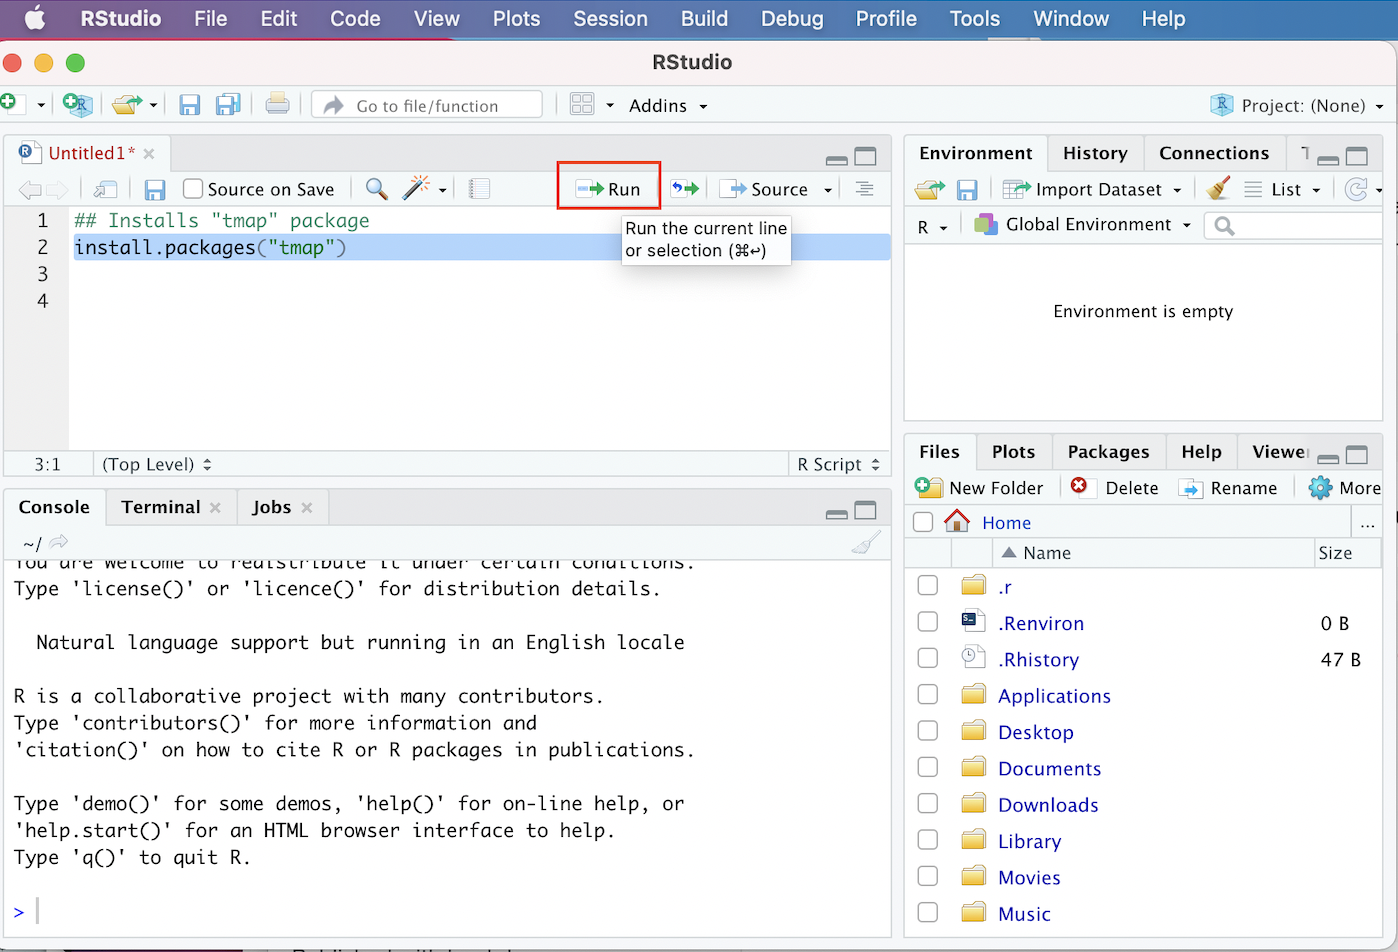
\includegraphics[width=1\linewidth]{images/script} \caption{The R Studio Interface}\label{fig:unnamed-chunk-3}
\end{figure}

Please note that you can follow along with the tutorial on your own computers by transferring all of the subsequent codeblocks into your script in just this way. Run each codeblock in your R Studio environment as you go, and you should be able to replicate the entire tutorial on your computer.

You'll note that the codeblocks in the tutorial usually have a comment, prefaced by a hash (``\#''). When writing code in R (or any other command-line interface) it is good practice to preface your code with brief comments that describe what a block of code is supposed to do. Writing these comments can allow someone else (or your future self) read and understand your code more easily than otherwise might be the case. The hash before the comment effectively tells R that the subsequent text is a comment, and should not be run as part of the subsequent code. If you didn't preface the comment with a hash, R wouldn't know to ignore the comment when executing the code, and would throw an error message.

Now, let's install the other packages we mentioned above, using the same function:

\begin{Shaded}
\begin{Highlighting}[]
\CommentTok{\# Installs remainder of necessary packages to complete exercise}
\FunctionTok{install.packages}\NormalTok{(}\StringTok{"sf"}\NormalTok{)}
\FunctionTok{install.packages}\NormalTok{(}\StringTok{"rnaturalearth"}\NormalTok{)}
\FunctionTok{install.packages}\NormalTok{(}\StringTok{"rnaturalearthdata"}\NormalTok{)}
\FunctionTok{install.packages}\NormalTok{(}\StringTok{"rgeos"}\NormalTok{)}
\FunctionTok{install.packages}\NormalTok{(}\StringTok{"readxl"}\NormalTok{)}
\FunctionTok{install.packages}\NormalTok{(}\StringTok{"dplyr"}\NormalTok{)}
\end{Highlighting}
\end{Shaded}

All of the packages we need are now installed!

\hypertarget{load-libraries}{%
\subsection{Load Libraries}\label{load-libraries}}

However, while our packages are installed in our R environment, they are not yet ready to use. Before we can use our packages, we must load them into our environment. You can think of the process of loading installed packages into a current R environment as analgous to opening up an application on your phone or computer after it has been installed (even if an application is installed, you can't use it until you open it!). To load (i.e.~``open'') an R package, we pass the name of the package we want to load as an argument to the \texttt{library} function. For example, if we want to load the ``tmap'' package into the current environment, we can type:

\begin{Shaded}
\begin{Highlighting}[]
\CommentTok{\# Loads "tmap" package}
\FunctionTok{library}\NormalTok{(tmap)}
\end{Highlighting}
\end{Shaded}

At this point, the full suite of the \emph{tmap} package's functionality is available for us to use.

Now, let's go ahead and load the remainder of the packages that we'll need:

\begin{Shaded}
\begin{Highlighting}[]
\CommentTok{\# Loads remainder of packages}
\FunctionTok{library}\NormalTok{(sf)}
\FunctionTok{library}\NormalTok{(rnaturalearth)}
\FunctionTok{library}\NormalTok{(rnaturalearthdata)}
\FunctionTok{library}\NormalTok{(rgeos)}
\FunctionTok{library}\NormalTok{(tidyverse)}
\FunctionTok{library}\NormalTok{(readxl)}
\FunctionTok{library}\NormalTok{(dplyr)}
\end{Highlighting}
\end{Shaded}

At this point, the packages are loaded and ready to go! One important thing to note regarding the installation and loading of packages is that you only have to install packages once; after a package is installed, there is no need to subsequently reinstall it. However, you must load the packages you need (using the \texttt{library} function) every time you open a new R session. In other words, if you were to close R Studio at this point and open it up later, you would \textbf{not} need to install these packages again (Step 1a), but you \textbf{would} need to load the packages again (Step 1b).

\hypertarget{set-working-directory}{%
\subsection{Set Working Directory}\label{set-working-directory}}

Before we can bring our data into R Studio and get started with the tutorial, we have to specify that data's location on our computer. This step is known as setting one's working directory. Before setting your working directory, make sure you've downloaded the ICPSR dataset, and have placed it in a directory (i.e.~folder) on your computer that was specifically created to store this data (See Section 3.1 above for more on the data).

If you're unfamiliar with the concept of file paths, the easiest way to set your working directory is through the R Studio menu. To do so, follow these steps:

\begin{itemize}
\tightlist
\item
  First, Click on the ``Session'' button on the R Studio menu at the top of your screen, and then scroll down to the ``Set Working Directory'' button in the menu that opens up.
\item
  When you hover over this button, a subsidiary menu that contains a button that says ``Choose Directory'' will open; click this ``Choose Directory'' button.
\item
  In the dialog box that opens up, navigate to the directory that contains the ICPSR data, select it, and click ``Open''. At this point, your working directory should be set!
\end{itemize}

The graphic below demonstrates the process of setting one's working directory through R Studio's menus:

\begin{figure}
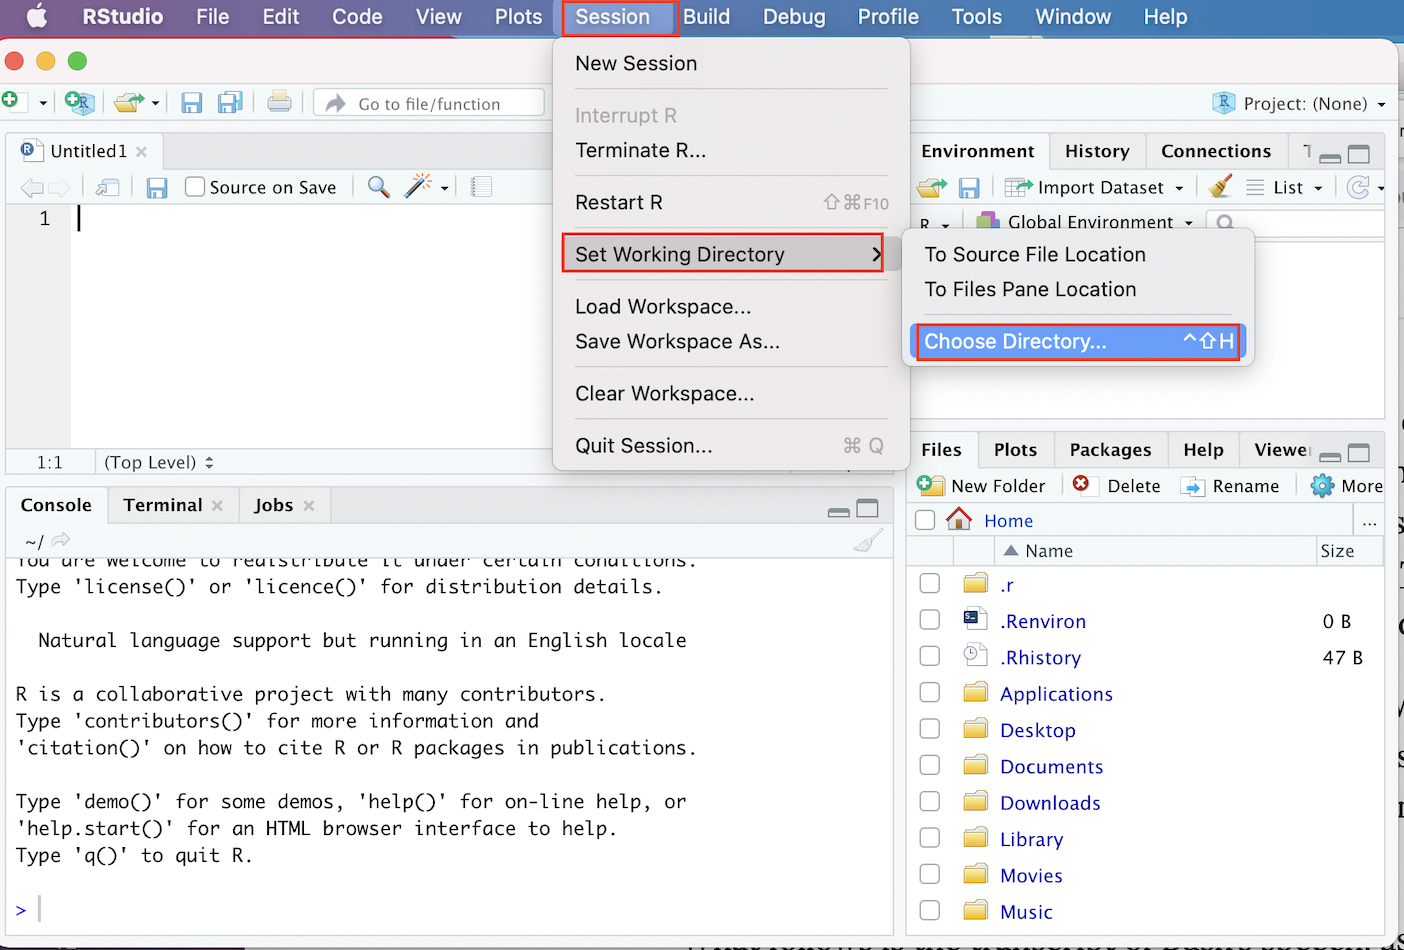
\includegraphics[width=1\linewidth]{images/setting_wd_revised} \caption{Setting Working Directory Via Menus}\label{fig:unnamed-chunk-7}
\end{figure}

\textbf{Alternatively}, if you are familiar with the concept of file paths, and know the file path to the folder containing the downloaded ICPSR dataset, you can set the working directly using the \texttt{setwd()} function, where the argument to the function is the relevant file path enclosed in quotation marks. For example:

\begin{Shaded}
\begin{Highlighting}[]
\CommentTok{\# Sets working directory }
\FunctionTok{setwd}\NormalTok{(}\StringTok{"/Users/adityaranganath/Documents/git\_repositories/icpsr\_mapping\_manual/tutorial\_data"}\NormalTok{)}
\end{Highlighting}
\end{Shaded}

Note that you won't want to copy and paste the above codeblock, since your file path will be different; be sure to replace your own file path with the one given above.

\hypertarget{tutorial}{%
\section{Tutorial}\label{tutorial}}

\hypertarget{load-and-view-data}{%
\subsection{Load and View Data}\label{load-and-view-data}}

Now that we've taken care of those preliminary steps, let's bring in the tutorial data into our R environment so that we can begin working with it. There are two pieces of data we'll need to load:

\begin{itemize}
\tightlist
\item
  The ICPSR tabular dataset on government policy responses to Covid-19 (Section 4.1.1)
\item
  A spatial dataset of world country boundaries; we will bring this dataset into R Studio via the \texttt{ne\_countries} function of the ``rnaturalearth'' package (Section 4.1.2)
\end{itemize}

\hypertarget{icpsr-covid-19-tabular-data}{%
\subsubsection{ICPSR Covid-19 Tabular Data}\label{icpsr-covid-19-tabular-data}}

When importing tabular data that you have saved on our computer into R Studio, it's important to first understand some of the details of the data we're trying to import. The first thing to note is the type of file we're working with, which is indicated by the file extension; here, we can note that the ICPSR data is a .xlsx file, which means that it's an Excel file (but note that .xlsx files can also be opened in spreadsheet software programs other than Excel). That means we'll have to import it into R Studio using a function designed specifically to handle Excel files. To that end, we'll use the \texttt{read\_excel} function from the \emph{readxl} package. Recall that if you want to learn more about a function or a package, simply type a question mark followed by the package or function name in the console, and relevant information will appear in the ``Help'' tab of the ``Files/Plots/Packages/Help/Viewer'' window on the bottom right of our R Studio interface. For example, if we wanted to learn more about the \texttt{read\_excel}function, we would type \texttt{?read\_excel} into the console.

Before using the \texttt{read\_excel} function to bring in the , it could be helpful to open up the data outside the R environment to see whether the dataset has any features that we have to account for when loading it into our R environment. When we first open the spreadsheet, it will look something like this:

\begin{figure}
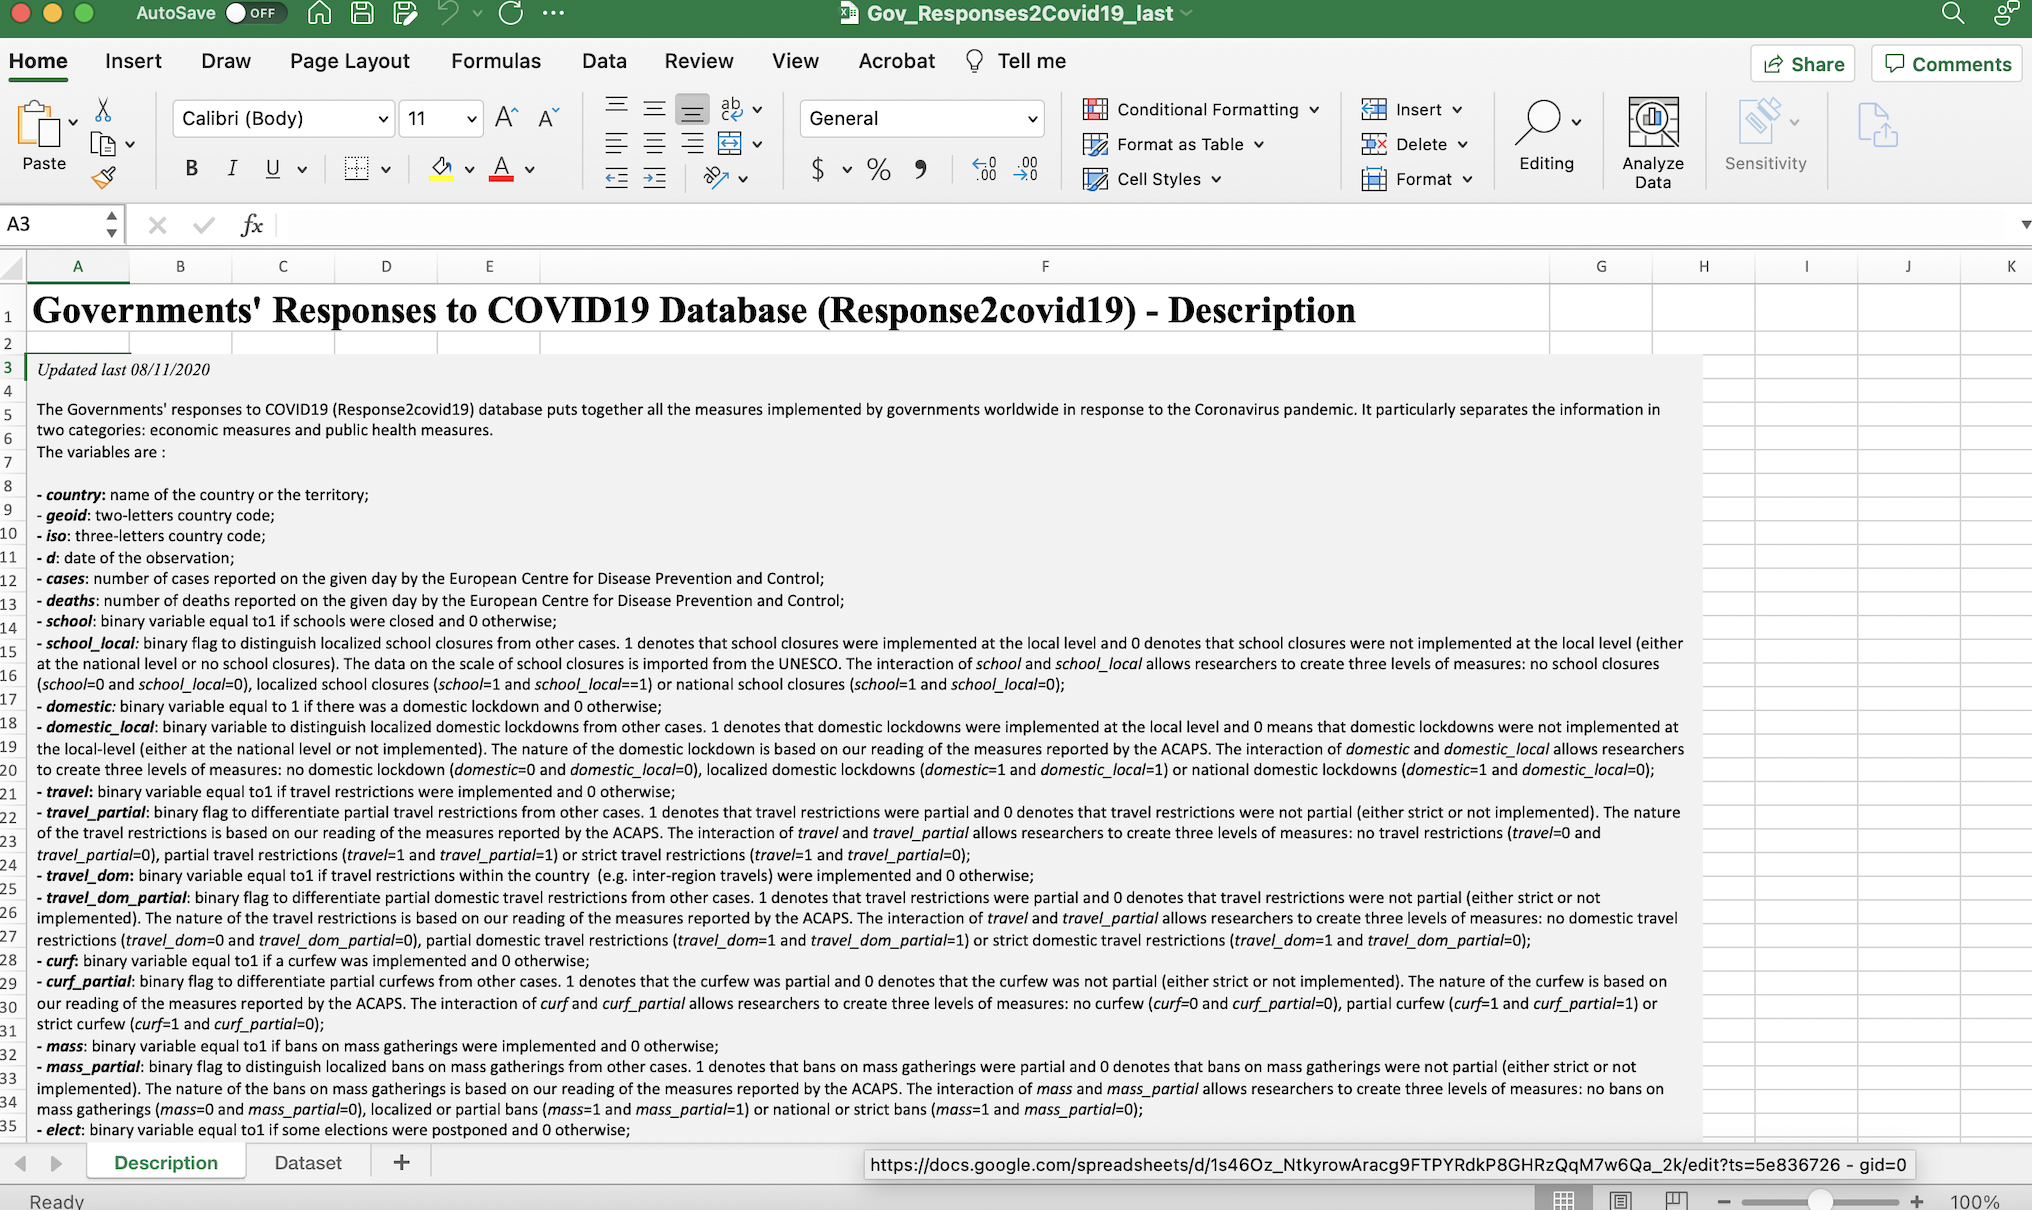
\includegraphics[width=1\linewidth]{images/excel_open} \caption{ICPSR Dataset in Spreadsheet: Description Tab}\label{fig:unnamed-chunk-10}
\end{figure}

Note that when we open the spreadsheet, we land on its first tab (or ``sheet''), which is titled ``Description''. This part of the spreadsheet effectively functions as a data codebook, which we can look through to understand the dataset's various variables and and assess how they were measured. To open up the actual dataset, we can toggle to the ``Dataset'' tab by pressing the corresponding button on the bottom-left of the spreadsheet (highlighted in red below):

\begin{figure}
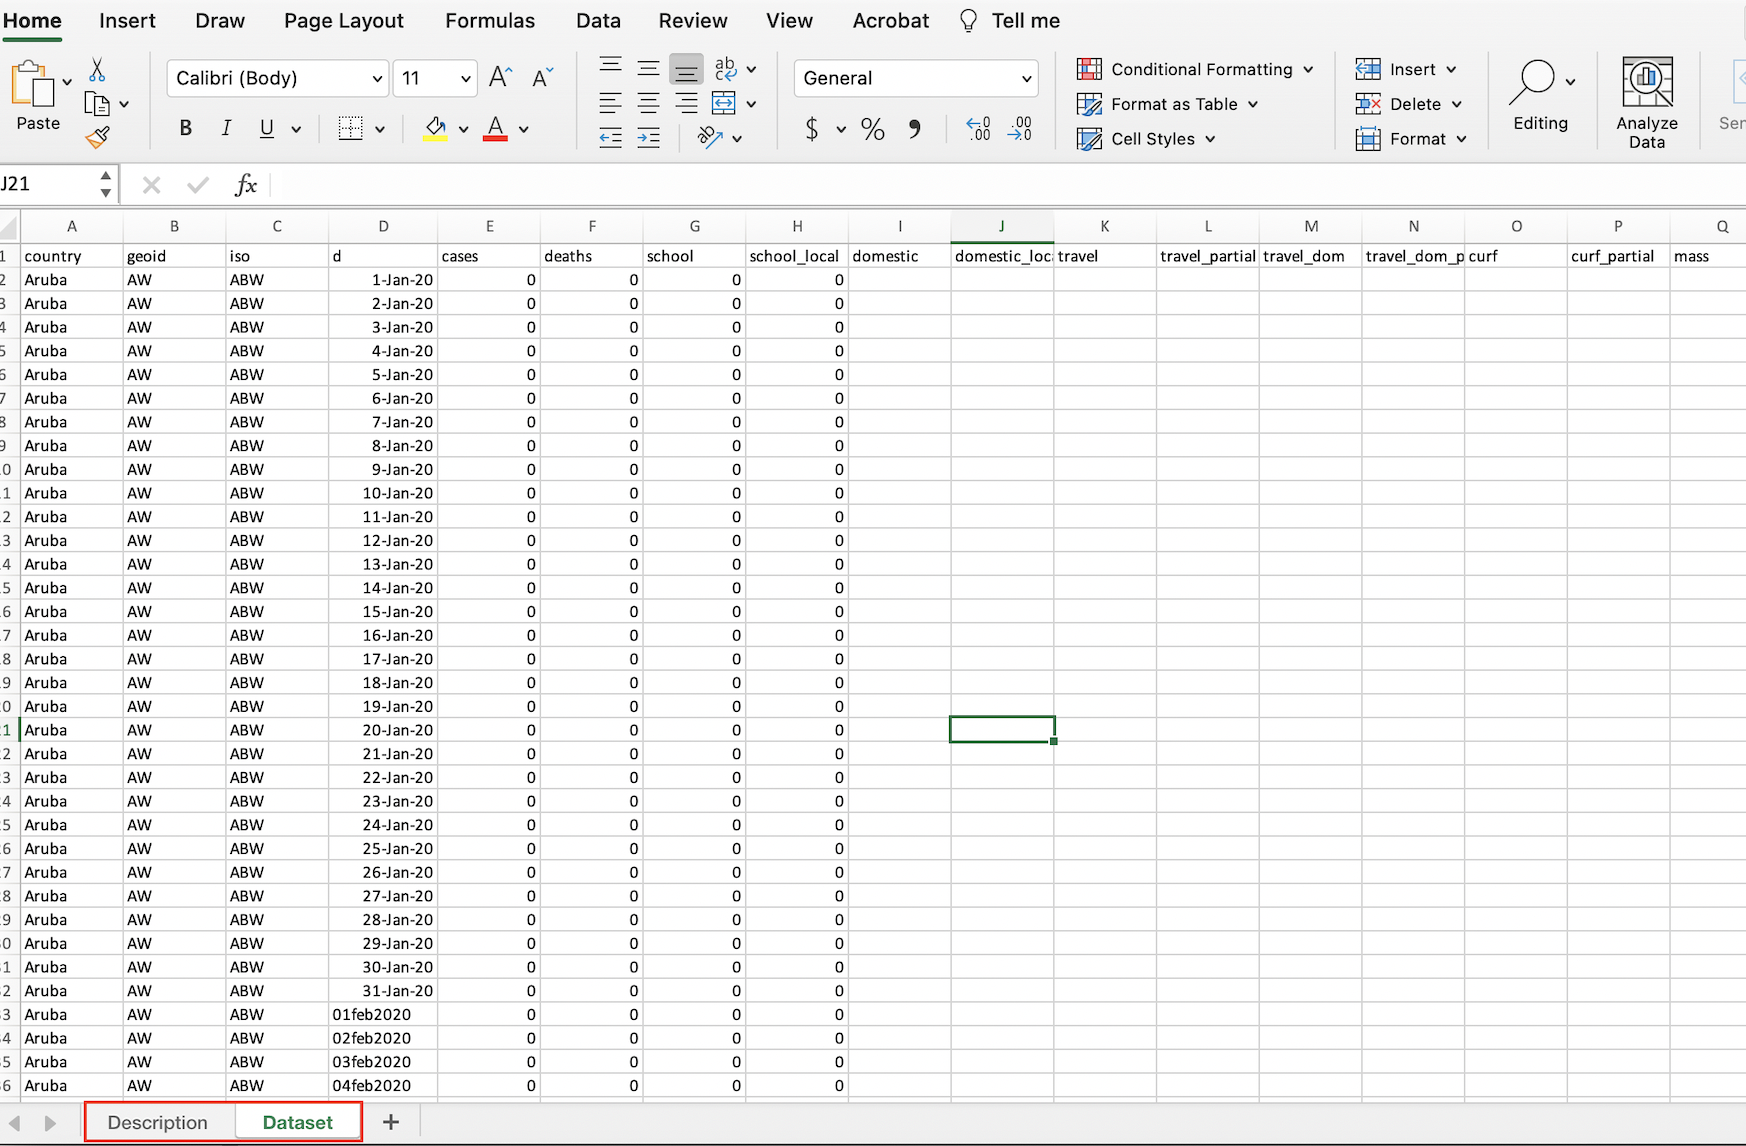
\includegraphics[width=1\linewidth]{images/excel_tabs} \caption{ICPSR Dataset in Spreadsheet: Dataset Tab}\label{fig:unnamed-chunk-11}
\end{figure}

The fact that the ICPSR dataset has two sheets within it is important; it means that when we load it into R, we'll have to explicitly specify the sheet (i.e.~the ``Dataset'' sheet) we want to import.

Now, let's go ahead and load the ``Dataset'' sheet of the ICPSR data file. Type the following code into your script, and run it:

\begin{Shaded}
\begin{Highlighting}[]
\CommentTok{\# Imports "Dataset" sheet from ICPSR Excel file into R Studio, and assigns the dataset to an object called "covid\_data"}
\NormalTok{covid\_data}\OtherTok{\textless{}{-}}\FunctionTok{read\_excel}\NormalTok{(}\StringTok{"Gov\_Responses2Covid19\_last.xlsx"}\NormalTok{, }\AttributeTok{sheet=}\StringTok{"Dataset"}\NormalTok{)}
\end{Highlighting}
\end{Shaded}

Let's unpack that code. As we noted above, \texttt{read\_excel} is the function used to bring in Excel spreadsheet data into R. The function has two arguments; the first (``Gov\_Responses2Covid19\_last.xlsx'') is the name of the file we want to import, while the second (sheet=``Dataset'') specifies that we specifically want to import the the ``Dataset'' sheet from that Excel file. This code is then assigned, using \texttt{\textless{}-} (R's assignment operator) to a new object that we call \texttt{covid\_data}. This means that the output of the code on the right hand side of the assignment operator is now assigned to the \texttt{covid\_data} object. Think of this object as a container of sorts, one which holds, or ``contains'', the output of the code to the right of the assignment operator. Object assignment isn't necessary; we could have brought the data into R Studio by simply typing the code to the right of the assignment operator. However, assigning the dataset to an object allows for the more flexible and intuitive handling of data, so it is a common practice.

Note that after typing the code from the previous codeblock into your R script and running it, you still won't actually see the dataset within the R environment. There are many ways to pull up and inspect the data; in this tutorial, we'll use the \texttt{View} function, which will bring up the data as a separate tab in the ``Source'' window. To display the contents of the \texttt{covid\_data} object (in other words, the dataset we just imported), type and run the following code:

\begin{Shaded}
\begin{Highlighting}[]
\CommentTok{\# Brings up dataset held in the "covid\_data" object in R Studio\textquotesingle{}s data viewer}
\FunctionTok{View}\NormalTok{(covid\_data)}
\end{Highlighting}
\end{Shaded}

Within your R Studio environment, the result of running \texttt{View(covid\_data)} will look something like this (dataset outlined in red):

\begin{figure}
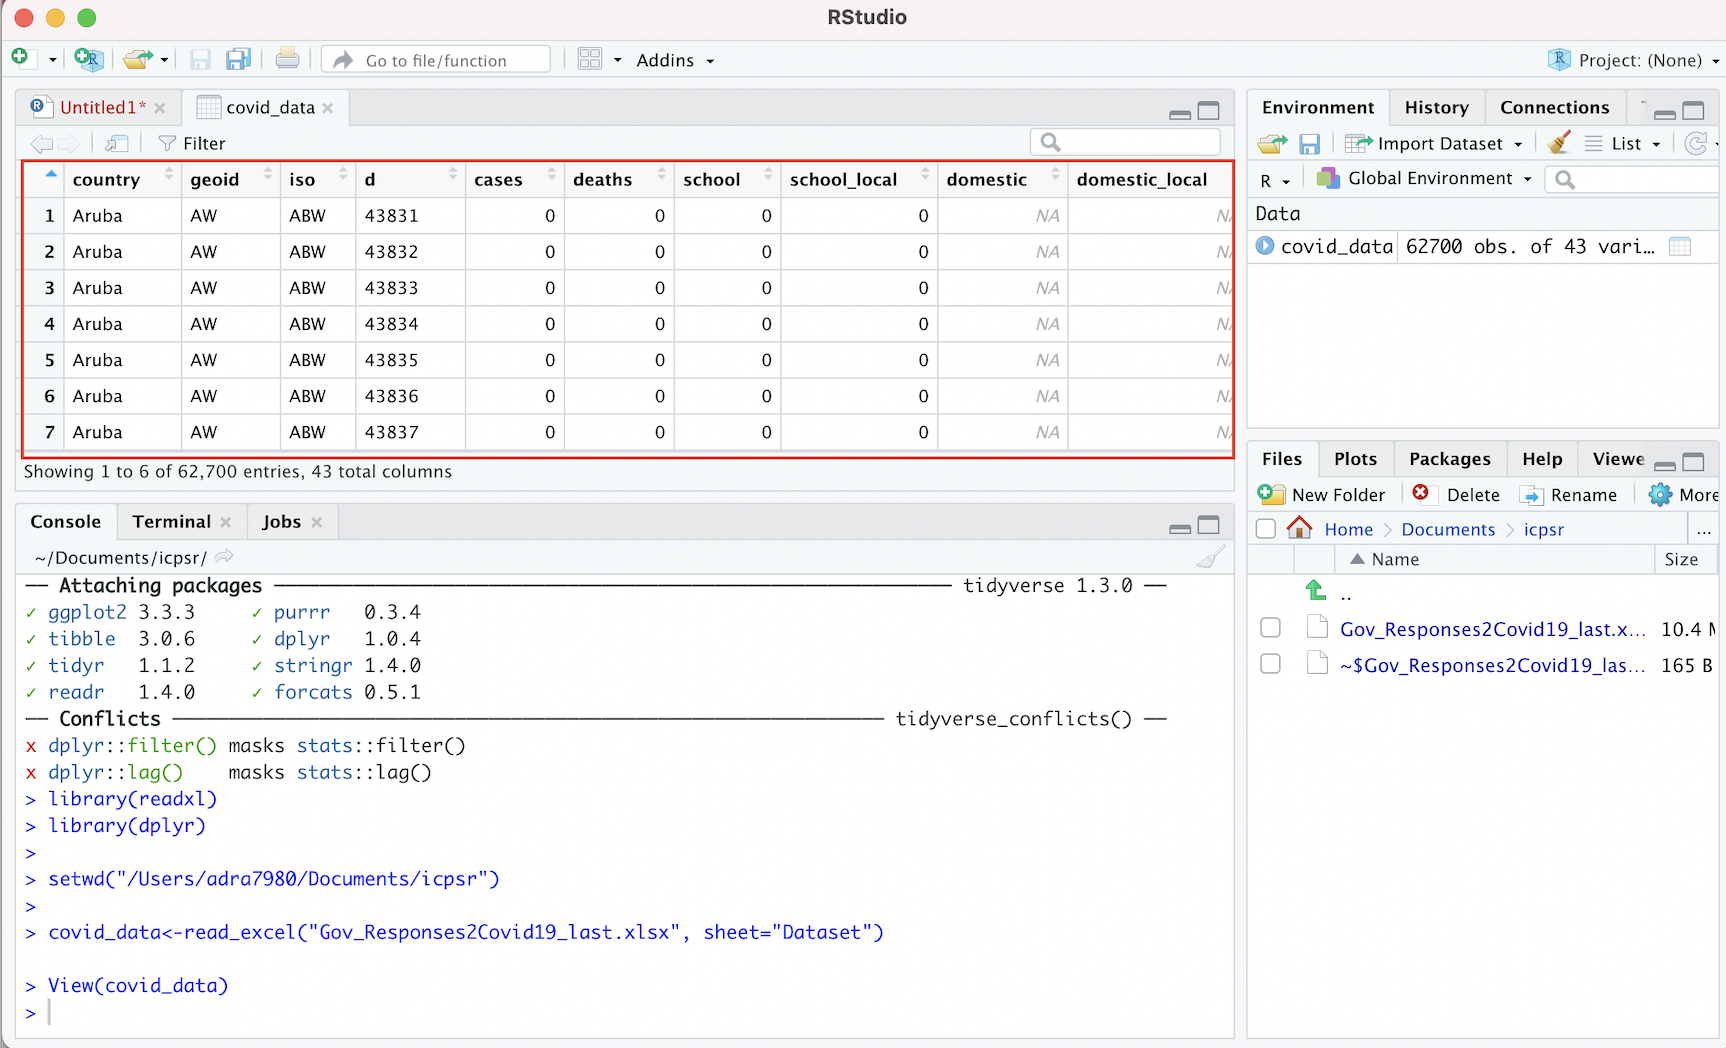
\includegraphics[width=1\linewidth]{images/viewdata} \caption{Viewing ICPSR Dataset in R Environment}\label{fig:unnamed-chunk-14}
\end{figure}

You can scroll up/down and across the dataset within the data viewer.

\hypertarget{country-boundaries-spatial-data}{%
\subsubsection{Country Boundaries Spatial Data}\label{country-boundaries-spatial-data}}

Now that we have our tabular data on government responses to Covid-19 loaded into R Studio, let's bring spatial data on world country borders into memory. Eventually, we'll represent the Covid-19 data on a map by joining it to the spatial data on country boundaries that we will now bring in.

When working with spatial data in R, you will sometimes want to import data that you collected on your own, or data that you downloaded. There are several functions in the \texttt{sf} package that will allow you to easily import your external spatial data in R; if you need to do this, you should consult the package's documentation.

In our case, we won't have to download and import the spatial data we need into R Studio, since there are R packages that already contain this spatial data. In particular, we'll use the \texttt{ne\_countries} function of the \emph{rnaturalearth} package to bring the country border dataset into our R environment. Note the two arguments we pass into the \texttt{ne\_countries} function: the ``scale'' argument specifies that we want to use a medium scale when rendering the map (the other options are `small' and `large'), while the ``returnclass'' argument specifies that we want the spatial dataset in `sf' format, which is a spatial data format that works well with the \emph{tmap} mapping package we'll use later. As in the previous section, we'll assign the dataset to an object so that we can easily work with it later; we'll call this object ``country\_boundaries'':

\begin{Shaded}
\begin{Highlighting}[]
\CommentTok{\# Brings spatial dataset of country boundaries into R environment using the rnaturalearth package}
\NormalTok{country\_boundaries}\OtherTok{\textless{}{-}}\FunctionTok{ne\_countries}\NormalTok{(}\AttributeTok{scale=}\StringTok{"medium"}\NormalTok{, }\AttributeTok{returnclass=}\StringTok{"sf"}\NormalTok{)}
\end{Highlighting}
\end{Shaded}

Now that we have this spatial dataset in memory and assigned to an object, let's step back and clarify what exactly a spatial dataset is. In some respects, a spatial dataset is like a typical tabular dataset. To see this, let's pass the ``country\_boundaries'' object through the \texttt{View()} function to open up the dataset:

\begin{Shaded}
\begin{Highlighting}[]
\FunctionTok{View}\NormalTok{(country\_boundaries)}
\end{Highlighting}
\end{Shaded}

By scrolling across the dataset, you'll notice that each row corresponds to a country, and that there are many columns that correspond to various country-level attributes. The key column, however, which makes this a spatial dataset (as opposed to merely a tabular one), is the information contained in a column called ``geometry''. This column contains geographic coordinate information that essentially defines a polygon for each country in the dataset. The ``geometry'' column is likely one of the last columns in the dataset, so you may have to scroll a bit to find it. Alternatively, we can use the \texttt{relocate} function in the \emph{dplyr} package to make the ``geometry'' column the first column in the dataset within ``country\_boundaries'', and then view this reordered dataset using the \texttt{View} function. The first argument passed to the \texttt{relocate} function (``country\_boundaries'') indicates the object that contains the relevant dataset, and the second argument ("geometry) indicates the name of the column we want to move to the front of the dataset.

\begin{Shaded}
\begin{Highlighting}[]
\FunctionTok{View}\NormalTok{(}\FunctionTok{relocate}\NormalTok{(country\_boundaries, geometry))}
\end{Highlighting}
\end{Shaded}

After typing in that code and running it in your script, the window with the reordered dataset should appear in your source window; note the ``geometry'' tab:

\begin{figure}
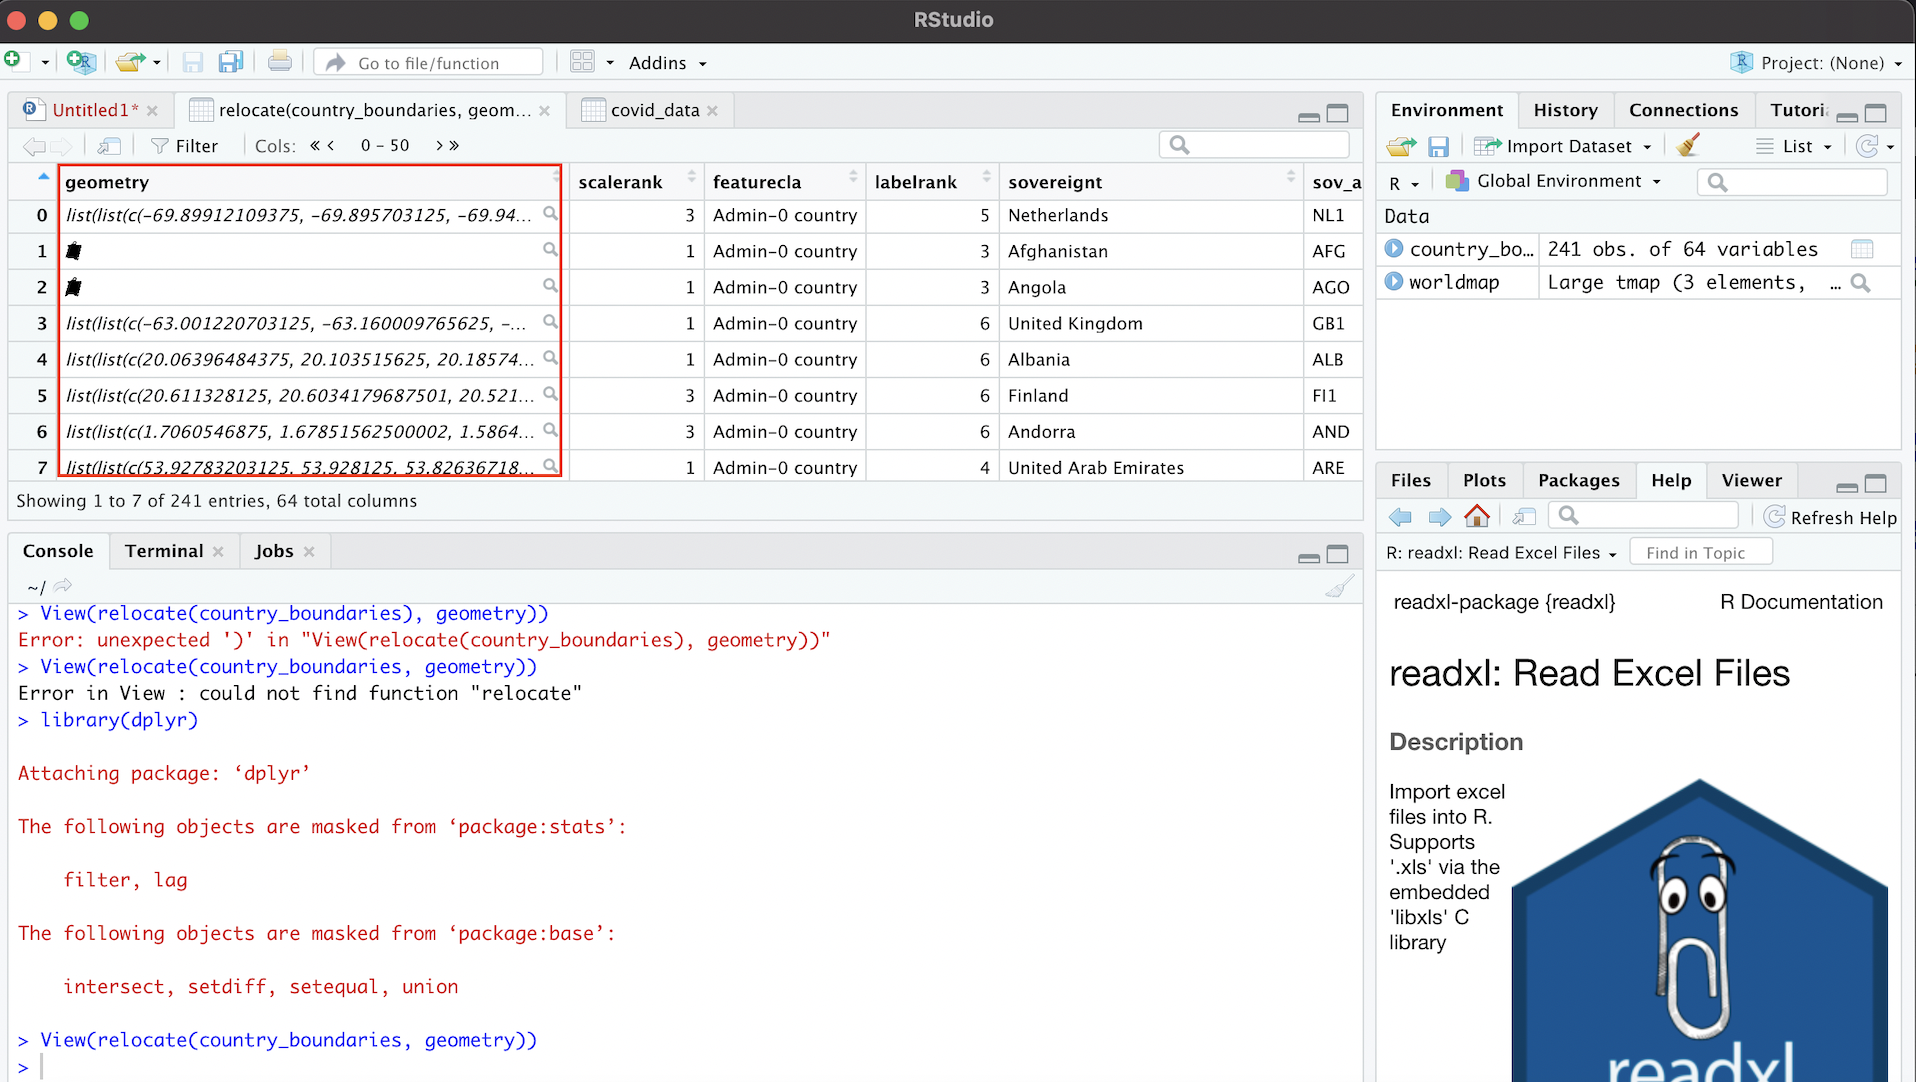
\includegraphics[width=1\linewidth]{images/geometry} \caption{Geometry Column Contains Spatial Information}\label{fig:unnamed-chunk-18}
\end{figure}

We can use the information in the ``geometry'' tab to draw georeferenced polygons for each row in the spatial dataset, which will yield a world map! To translate the information in the geometry tab into a cartographic representation, we'll use a package called \emph{tmap}. To bring up the features of the dataset, we have to first tell \emph{tmap} what dataset contains the information we want to map; we do this by first passing the name of the object that contains the relevant dataset (here, ``country\_boundaries'') to the \texttt{tm\_shape} function, and then specifying that our features (i.e.~country borders) are represented as polygons through the \texttt{tm\_polygons} function. The \texttt{tm\_polygons} function does not require any arguments. In the \emph{tmap} package, we can connect functions together through a plus sign (+). When we type in and run the following code, the result is a map that is rendered based on the information in the ``geometry'' column:

\begin{Shaded}
\begin{Highlighting}[]
\CommentTok{\# maps geographic features (i.e. countries) of spatial dateset}
\FunctionTok{tm\_shape}\NormalTok{(country\_boundaries)}\SpecialCharTok{+}
  \FunctionTok{tm\_polygons}\NormalTok{()}
\end{Highlighting}
\end{Shaded}

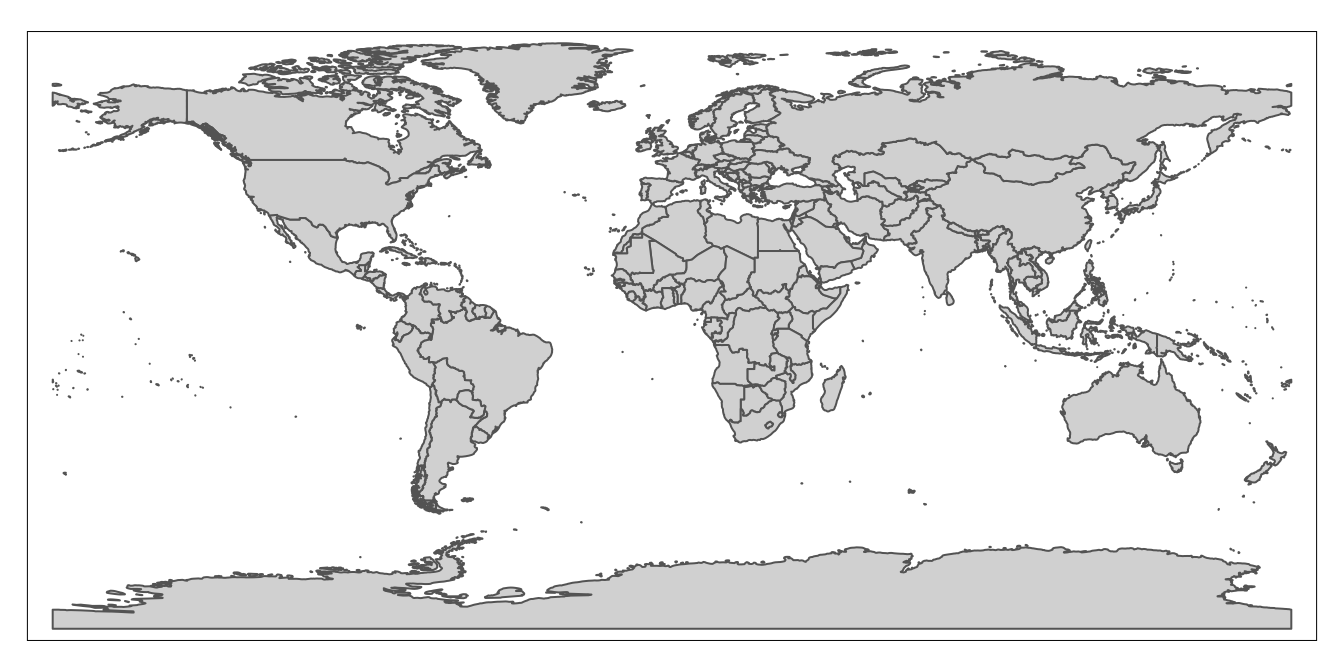
\includegraphics{bookdownproj_files/figure-latex/unnamed-chunk-19-1.pdf}

We can assign this map to an object, just as we assigned the ICPSR tabular dataset to an object. Let's call this object ``worldmap.''

\begin{Shaded}
\begin{Highlighting}[]
\CommentTok{\# assigns map of geographic features to a new object called "worldmap" }
\NormalTok{worldmap}\OtherTok{\textless{}{-}}\FunctionTok{tm\_shape}\NormalTok{(country\_boundaries)}\SpecialCharTok{+}
            \FunctionTok{tm\_polygons}\NormalTok{()}
\end{Highlighting}
\end{Shaded}

Having assigned the map to the ``worldmap'' object, we can bring up the map whenever we want by simply calling ``worldmap'' object: t:

\begin{Shaded}
\begin{Highlighting}[]
\CommentTok{\# calls "worldmap" object to display country{-}level map generated from the "country\_boundaries" spatial dataset }
\NormalTok{worldmap}
\end{Highlighting}
\end{Shaded}

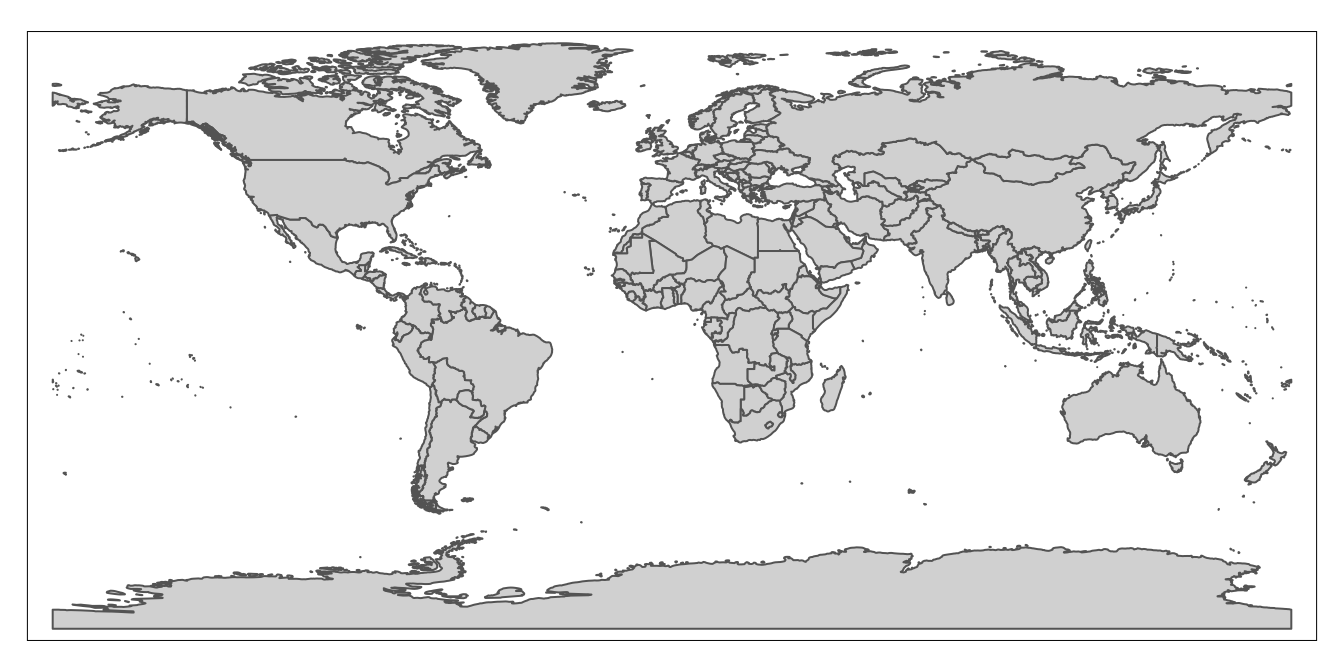
\includegraphics{bookdownproj_files/figure-latex/unnamed-chunk-21-1.pdf}

Within the R Studio interface, we can see the above map within the bottom-right window after selecting the ``Plots'' tab:

\begin{figure}
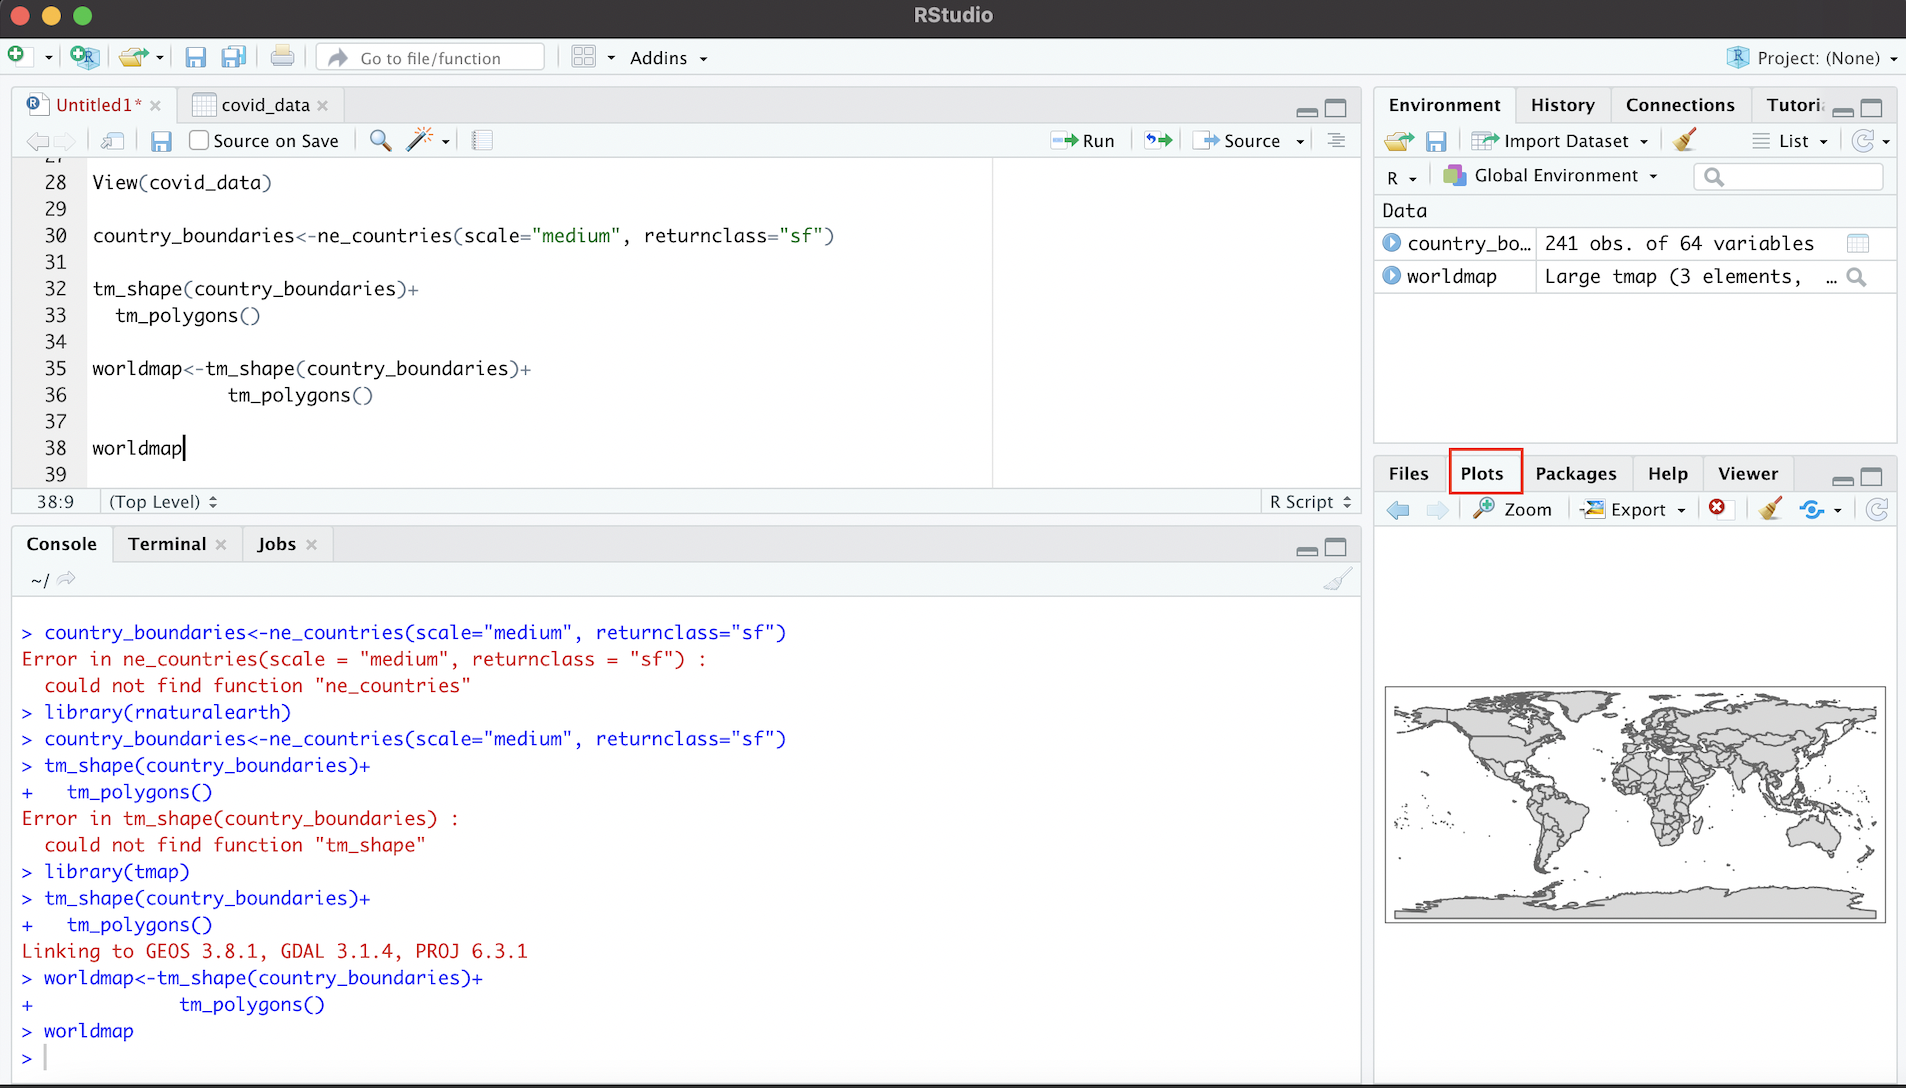
\includegraphics[width=1\linewidth]{images/worldmap_window} \caption{World Map in "Plots" Tab (Rendered from Spatial Dataset}\label{fig:unnamed-chunk-22}
\end{figure}

We can enlarge the map in this window by clicking the ``Zoom'' link; this will produce an enlarged version of the map in a separate window:

\begin{figure}
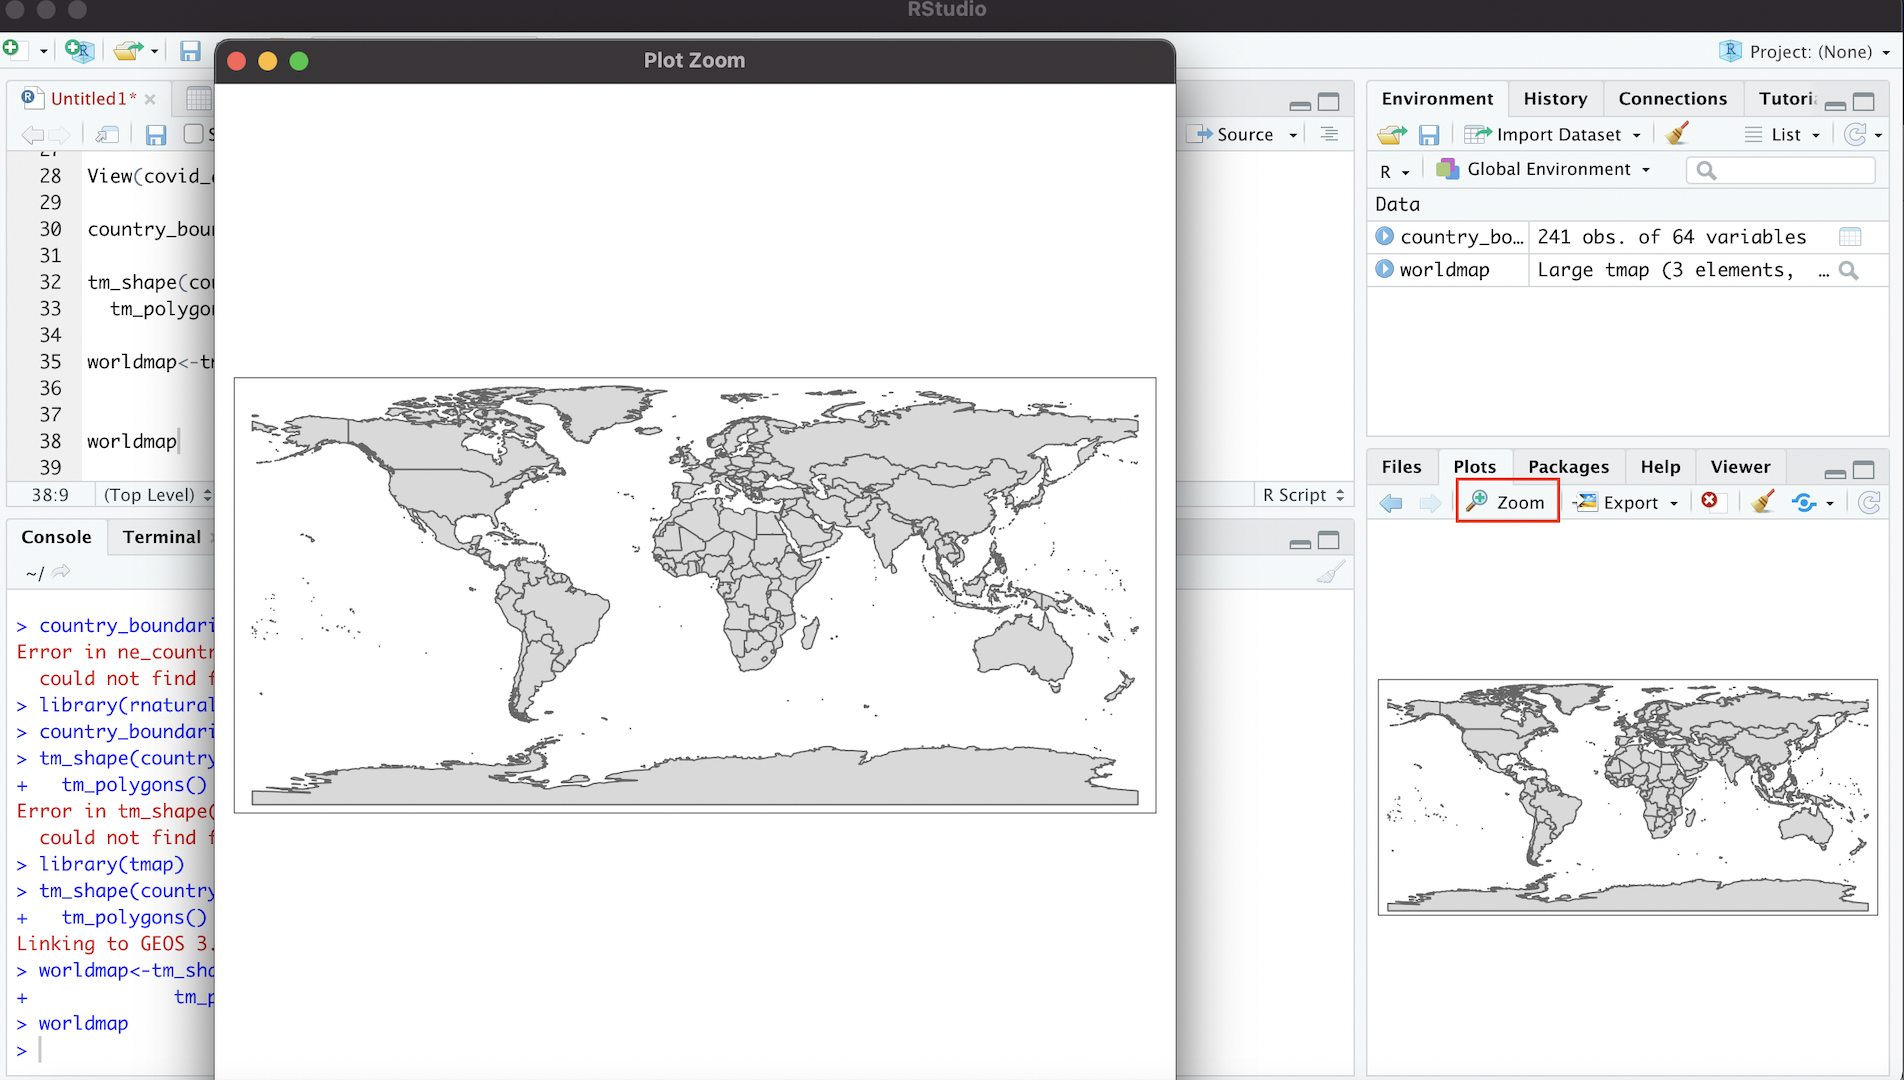
\includegraphics[width=1\linewidth]{images/zoom2} \caption{Enlarging Map with "Zoom" Button}\label{fig:unnamed-chunk-23}
\end{figure}

\hypertarget{edit-spatial-data}{%
\subsection{Edit Spatial Data}\label{edit-spatial-data}}

We can edit spatial datasets in R Studio with relative ease, using commonly used R packages. Let's say, for example, that we don't want Antarctica to appear on our map (since Antarctica typically does not appear on political maps of the world).

To delete Antarctica from the map, we first need to delete the row that corresponds to Antarctica from the spatial dataset contained in the ``country\_boundaries'' object. We can do so with the following code:

\begin{Shaded}
\begin{Highlighting}[]
\CommentTok{\# Deletes Antarctica from spatial dataset in "country\_boundaries" object}
\NormalTok{country\_boundaries}\OtherTok{\textless{}{-}}\NormalTok{country\_boundaries }\SpecialCharTok{\%\textgreater{}\%} \FunctionTok{filter}\NormalTok{(iso\_a3 }\SpecialCharTok{!=}\StringTok{"ATA"}\NormalTok{)}
\end{Highlighting}
\end{Shaded}

We can translate this code into ordinary language as follows: ``Take the existing country boundaries dataset (\texttt{country\_boundaries} to the left of the \texttt{\%\textgreater{}\%} and after the assignment operator) and then (\texttt{\%\textgreater{}\%}, a symbol called a pipe, which is used to chain together code) select only the countries that are not Antarctica (\texttt{filter(iso\_a3\ !="ATA"}). Take this new dataset, which doesn't include Antarctica, and assign it back to the existing `country\_boundaries' object (\texttt{country\_boundaries\textless{}-}), which effectively replaces the previous spatial dataset in the country\_boundaries object (which did include Antarctica).''

Two things may require additional elaboration:

\begin{itemize}
\tightlist
\item
  First is the pipe, the symbol that looks like this: \%\textgreater\%. The pipe operator essentially takes the output of the code on its left, and then use that output as an input to the code on its right. Here, the pipe is taking the output of the Here, the pipe is taking the output of the ``country\_dataset'' object (i.e.~the existing spatial dataset) on its left, and then using that output as an input to the \texttt{filter} function on its right. In other words, the pipe operator links the code on its two sides, and indicates that the object being passed through the \texttt{filter} function is the ``country\_boundaries'' object.
\item
  The \texttt{filter} function is a function from the \emph{dplyr} package that allows one to select rows from a dataset by specified criteria. In our case, we want to select all rows from the dataset that are not Antarctica. The argument to the \texttt{filter} function, \texttt{iso\_a3\ !="ATA"}, is essentially saying ``return any records where the iso\_a3 variable in the attribute table (the 3-digit ISO country code) is NOT equal to''ATA" (Antarctica's code). Note that \texttt{!=} is R syntax for ``not equal to''.\footnote{If we were to instead type \texttt{filter(iso\_a3=="ATA)}, the function would \emph{only} select the Antarctica row from the dataset and discard everything else.}
\end{itemize}

Now, let's see this change reflected in the corresponding map. To do so, we must update the ``worldmap'' object by rerunning the object assignment. The worldmap object we defined above will not automatically reflect the edits we just made to the ``country\_boundaries'' dataset; we need to run the code again with the edited version of the dataset ``country\_boundaries'' object passed through the \texttt{tm\_shape} function:

\begin{Shaded}
\begin{Highlighting}[]
\NormalTok{worldmap}\OtherTok{\textless{}{-}}\FunctionTok{tm\_shape}\NormalTok{(country\_boundaries)}\SpecialCharTok{+}
            \FunctionTok{tm\_polygons}\NormalTok{()}
\end{Highlighting}
\end{Shaded}

Now, let's view our updated map:

\begin{Shaded}
\begin{Highlighting}[]
\NormalTok{worldmap}
\end{Highlighting}
\end{Shaded}

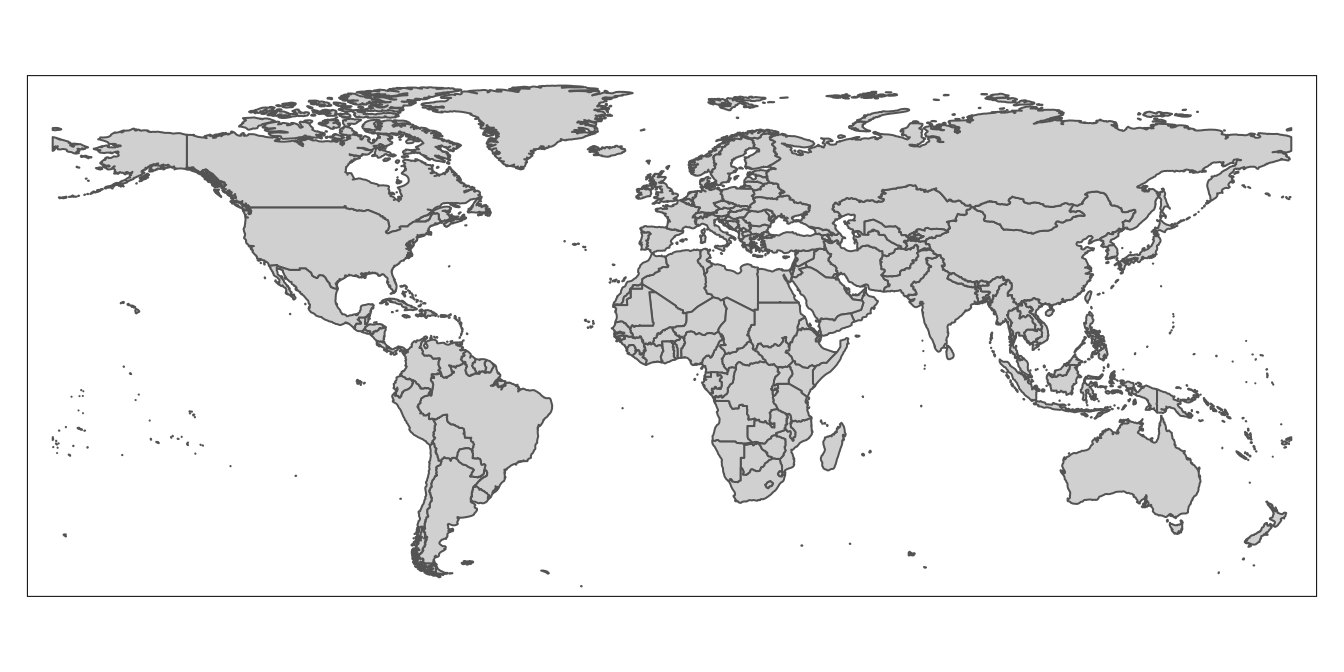
\includegraphics{bookdownproj_files/figure-latex/unnamed-chunk-26-1.pdf}

As desired, Antarctica has been deleted from the spatial dataset, and therefore no longer appears on the corresponding map.

\hypertarget{process-icpsr-tabular-data-for-mapping}{%
\subsection{Process ICPSR Tabular Data for Mapping}\label{process-icpsr-tabular-data-for-mapping}}

In order to represent the ICPSR data on governments' economic responses to Covid-19 on a map, we must join the ICPSR dataset (contained in the ``covid\_data'' object) to the spatial dataset (contained in the ``country\_boundaries'' object); at that point, we'll have a new, integrated dataset that will include the country-level Covid-19 data of interest in a spatial dataset. We can then display that Covid-19 information on a map by using the \texttt{tmap} package.
Before we can take those steps, however, we need to process the ICPSR tabular data with a view towards facilitating the joining and mapping process.

\hypertarget{select-variables}{%
\subsubsection{Select Variables}\label{select-variables}}

When working with data in R, it is often useful to get a quick sense of a given dataset's dimensions, which we can do using the \texttt{dim} function. Below, we pass the ``covid\_data'' object through the \texttt{dim} function:

\begin{Shaded}
\begin{Highlighting}[]
\FunctionTok{dim}\NormalTok{(covid\_data)}
\end{Highlighting}
\end{Shaded}

\begin{verbatim}
## [1] 62700    43
\end{verbatim}

The output indicates that there are 62700 rows in the dataset, and 43 columns. This suggests that there are quite a few variables in the dataset. Given that we're only interested in mapping (for now) the variable that represents an aggregate index (computed from other variables in the dataset) of the generosity of governments' economic support measures in response to the pandemic, we'll go ahead and delete superfluous columns so as to keep the size of the final (joined) dataset tractable. The name of the variable we'd like to map, and therefore keep, is ``Economic\_Measure'' (see the dataset's documentation for more details). In addition to keeping this variable, we also need to keep a column titled ``iso'', which is the 3-digit ISO country code; this ISO code also exists in the spatial dataset to which we want to join the ``Economic\_Measure'' variable, and so we will use these ISO codes as the joining variable.

Let's create a new object, which we'll call ``covid\_data\_economic'', to contain this smaller dataset comprised of the ISO code and the economic interventions index we're interested in mapping:

\begin{Shaded}
\begin{Highlighting}[]
\NormalTok{covid\_data\_economic}\OtherTok{\textless{}{-}}\NormalTok{covid\_data }\SpecialCharTok{\%\textgreater{}\%} 
                      \FunctionTok{select}\NormalTok{(iso, Economic\_Measures) }
\end{Highlighting}
\end{Shaded}

The above code can be translated as follows: ``Start with the dataset in the `covid\_data' object (`covid\_data'), and then keep the `iso' and `Economic\_Measures' columns but discard everything else (`select(iso, Economic\_Measures)). Assign this new 2-column dataset to a new object called 'covid\_data\_economic' (`covid\_data\_economic\textless-').'' We can take a look at this smaller dataset extracted from the original dataset by passing the ``covid\_data\_economic'' object as an argument to the now-familiar \texttt{View} function:

\begin{Shaded}
\begin{Highlighting}[]
\FunctionTok{View}\NormalTok{(covid\_data\_economic)}
\end{Highlighting}
\end{Shaded}

Within the ``Source'' window, a new tab that contains the smaller 2-column dataset that is within the ``covid\_data\_economic'' object will appear:

\begin{figure}
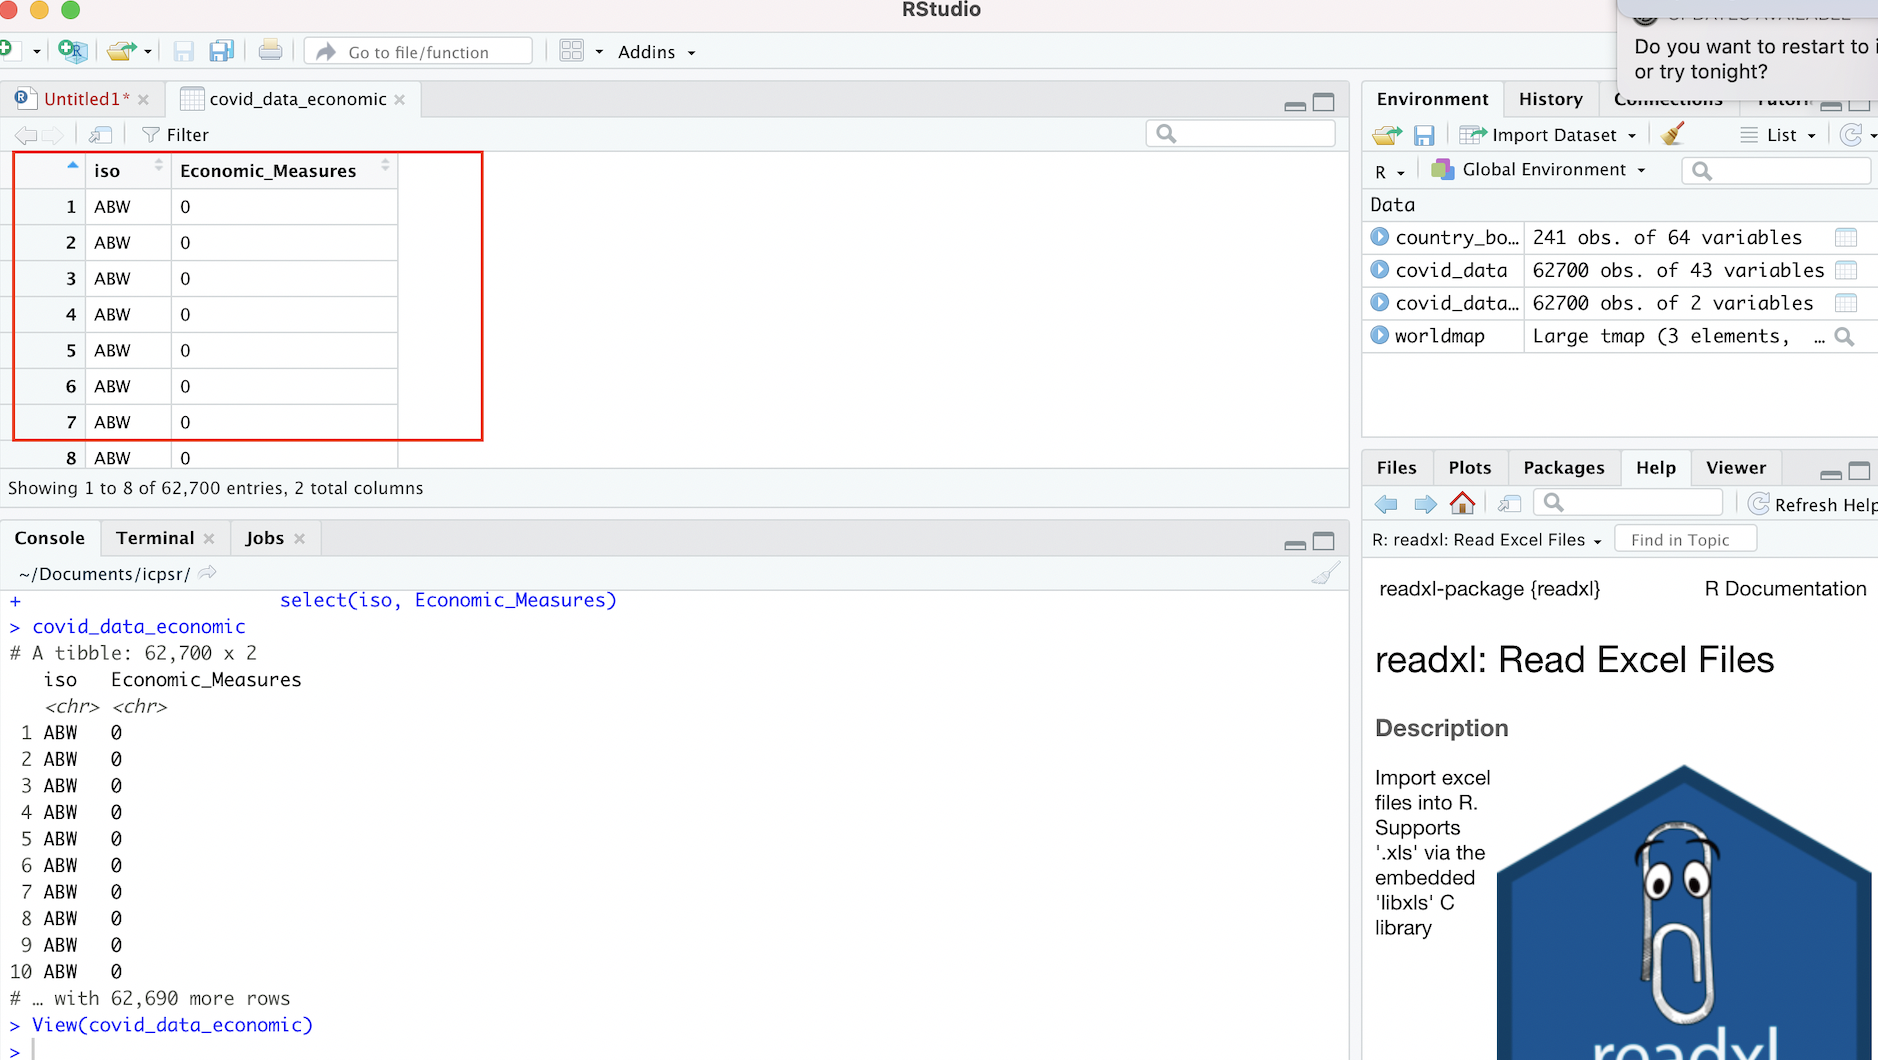
\includegraphics[width=1\linewidth]{images/selection} \caption{New Dataset Based on Selection from Original Dataset}\label{fig:unnamed-chunk-30}
\end{figure}

Note that the original Covid-19 policy responses dataset, stored in the ``covid\_data'' object, is unaffected by our creation of a new dataset based on the selection of these two variables. You can confirm that this original data is still stored in the ``covid\_data'' object by opening it up:

\begin{Shaded}
\begin{Highlighting}[]
\FunctionTok{View}\NormalTok{(covid\_data)}
\end{Highlighting}
\end{Shaded}

We can go back to this initial dataset (in the ``covid\_data'' object) anytime we might need, but for now we'll set it aside and start working with our newly created dataset in the ``covid\_data\_economic'' object.

\hypertarget{change-class-of-economic_measures-index}{%
\subsubsection{Change class of ``Economic\_Measures'' Index}\label{change-class-of-economic_measures-index}}

Recall that the data we want to map is contained within the ``Economic\_Measures'' field of the dataset in the newly created ``covid\_data\_economic'' dataset. R has six fundamental ``types'' of data: character, numeric, integer, logical, and complex. The code below extracts the ``Econmic\_Measures'' column from the dataset (placing a dollar sign in between the name of an object containing a dataset, and a column containing that dataset, as in \texttt{covid\_data\_economic\$Economic\_Measures} is a way of isolating and extracting a column from a larger dataset), and then passes it through the \texttt{class} function to identify the class of the ``Economic\_Measures'' field.

\begin{Shaded}
\begin{Highlighting}[]
\CommentTok{\# Find the class of the "Economic\_Measures" field}
\FunctionTok{class}\NormalTok{(covid\_data\_economic}\SpecialCharTok{$}\NormalTok{Economic\_Measures)}
\end{Highlighting}
\end{Shaded}

\begin{verbatim}
## [1] "character"
\end{verbatim}

We can see from the above output that the class of the ``Economic\_Measures'' variable is ``character'', which implies that although the information in the ``Economic\_Measures'' variable looks like it is numeric, R is not actually reading that data as numbers. So, we have to change the way that data is encoded, and ensure that it will be interpreted numerically; the failure to do this will prevent us from making numerical calculations using this data, as well as from mapping it using \emph{tmap}. We can essentially recode the information in the ``Economic\_Measures'' variable as ``numeric'' using the following code:

\begin{Shaded}
\begin{Highlighting}[]
\CommentTok{\# Changes class of "Economic\_Measures" field from character to numeric}
\NormalTok{covid\_data\_economic}\SpecialCharTok{$}\NormalTok{Economic\_Measures}\OtherTok{\textless{}{-}}\FunctionTok{as.numeric}\NormalTok{(covid\_data\_economic}\SpecialCharTok{$}\NormalTok{Economic\_Measures)}
\end{Highlighting}
\end{Shaded}

In the code above, the code to the right of the assignment operator extracts the ``Economic\_Measures'' column from the the ``covid\_data\_economic'' dataset, and then changes its class to numeric using the \texttt{as.numeric} function. The assignment operator then assigns this numeric version of the ``Economic\_Measures'' field back into the original dataset contained in the ``covid\_data\_economic'' object (the one with the character field); in performing this assignment, the ``character'' version of the ``Economic\_Measures'' field is replaced with the ``numeric'' version. At this point, the ``Economic\_Measures'' column in our dataset within the ``covid\_data\_economic'' object is numeric; we can confirm this by passing the column through the class function once again:

\begin{Shaded}
\begin{Highlighting}[]
\CommentTok{\# Find the class of the updated "Economic\_Measures" field}
\FunctionTok{class}\NormalTok{(covid\_data\_economic}\SpecialCharTok{$}\NormalTok{Economic\_Measures)}
\end{Highlighting}
\end{Shaded}

\begin{verbatim}
## [1] "numeric"
\end{verbatim}

\hypertarget{compute-average-of-economic_measures-index}{%
\subsubsection{Compute average of ``Economic\_Measures'' index}\label{compute-average-of-economic_measures-index}}

As we mentioned earlier, the ICPSR dataset on government policies with respect to Covid-19 is a time-series dataset, containing monthly observations over the course of about a year during the pandemic (January 2020 to October 2020). This means that we have to make some choices about how to represent the ``Economic\_Measures'' index on a map. For example, do we want to pick one of the months to map? Do we want to map the change across two different months? Do we want to map the average index value across all the months in the sample?

There are of many possibilities, but let's choose to go ahead and map the average. That is, for each country, we'll average the value of the ``Economic\_Measures'' index across all of the months in the dataset; the value that we'll eventually map will be this average value of the ``Economic\_Measures'' index.

To that end, we need to take our current ``covid\_data\_economic'', which contains monthly observations for each country, and transform it into a new dataset that contains the monthly average of the ``Economic\_Measures'' index for each country.

The code below carries out this transformation of the data:

\begin{Shaded}
\begin{Highlighting}[]
\CommentTok{\# Calculate Country{-}Level Averages for "Economic\_Measures" Index, and then assign this new dataset of country{-}level averages to a new object called "covid\_data\_economic\_avg". }
\NormalTok{covid\_data\_economic\_avg}\OtherTok{\textless{}{-}}\NormalTok{covid\_data\_economic }\SpecialCharTok{\%\textgreater{}\%} \FunctionTok{group\_by}\NormalTok{(iso) }\SpecialCharTok{\%\textgreater{}\%} 
                                                \FunctionTok{summarize}\NormalTok{(}\AttributeTok{mean\_economic=}\FunctionTok{mean}\NormalTok{(Economic\_Measures, }\AttributeTok{na.rm=}\ConstantTok{FALSE}\NormalTok{))}
\end{Highlighting}
\end{Shaded}

Let's unpack this code, starting with the code that's to the right of the assignment operator.

\begin{itemize}
\tightlist
\item
  We start by calling the ``covid\_data\_economic'' object, which establishes that this is essentially the ``base'' dataset we wish to modify.
\item
  Then (recall that the \texttt{\%\textgreater{}\%} is used to chain together code by taking the output on the left and passing it as input into the code to its right), we call the \texttt{group\_by} function, and pass ``iso'' as an argument to this function; this stipulates that all observations with the same ISO code are to be considered a group, and that any subsequent calculations will therefore be performed at the country level. This step ensures that when we calculate the mean of the ``Economic\_Measures'' variable, the function will return the mean value of this index for each individual country, rather than the mean value for the dataset as a whole.
\item
  After setting the grouping variable and using another pipe (\texttt{\%\textgreater{}\%}) to establish that we are passing the newly grouped dataset as an input into the subsequent code, we call the \texttt{summarize} function. This function creates a new dataset based on the calculation of summary statistics for an existing dataset. By calling \texttt{summarize}, we are specifying that we want to create a new dataset to hold the information on country-level averages for the ``Economic\_Measures'' data.
\item
  Within the \texttt{summarize} function, we first need to create a name for the column that will contain the country-level averages for the ``Economic\_Measures'' index. We'll call this variable ``mean\_economic'', which corresponds to the very first part of the code after the parentheses. We set this variable equal to an expression that passes the ``Economic\_Measures'' variable through the \texttt{mean} function. In essence, this calculates the mean of the ``Economic\_Measures'' variable for each country (it calculates the country-level mean because we specified the grouping function, \texttt{group\_by(iso)}, in the previous line of code), and creates a column in the newly created dataset named ``mean\_economic'' to store this information. The code that reads \texttt{na.rm=FALSE} simply specifies that missing data should be ignored in the calculation of the mean value of the ``Economic\_Measures'' index.
\item
  Finally, the this new dataset, consisting of two columns (one column containing ISO codes, and the other, named ``mean\_economic'' containing the corresponding country-level mean of the ``Economic\_Measures'' variable) is assigned to a new object called ``covid\_data\_economic\_avg''.
\end{itemize}

We can translate the above code as follows: ``Take the existing dataset within the `covid\_data\_economic' object, and then group this dataset by the ISO country codes; then, generate a new dataset, containing one column with ISO country codes, and another column, named''mean\_economic``, that contains information on the country-level mean of the `Economic\_Measures' index. Finally, assign this new dataset to an object called `covid\_data\_economic\_avg'\,''

To inspect this new dataset within the Source window, simply pass the object through the \texttt{View} function.

\begin{Shaded}
\begin{Highlighting}[]
\FunctionTok{View}\NormalTok{(covid\_data\_economic\_avg)}
\end{Highlighting}
\end{Shaded}

We should see something that looks like this:

\textbackslash begin\{figure\}
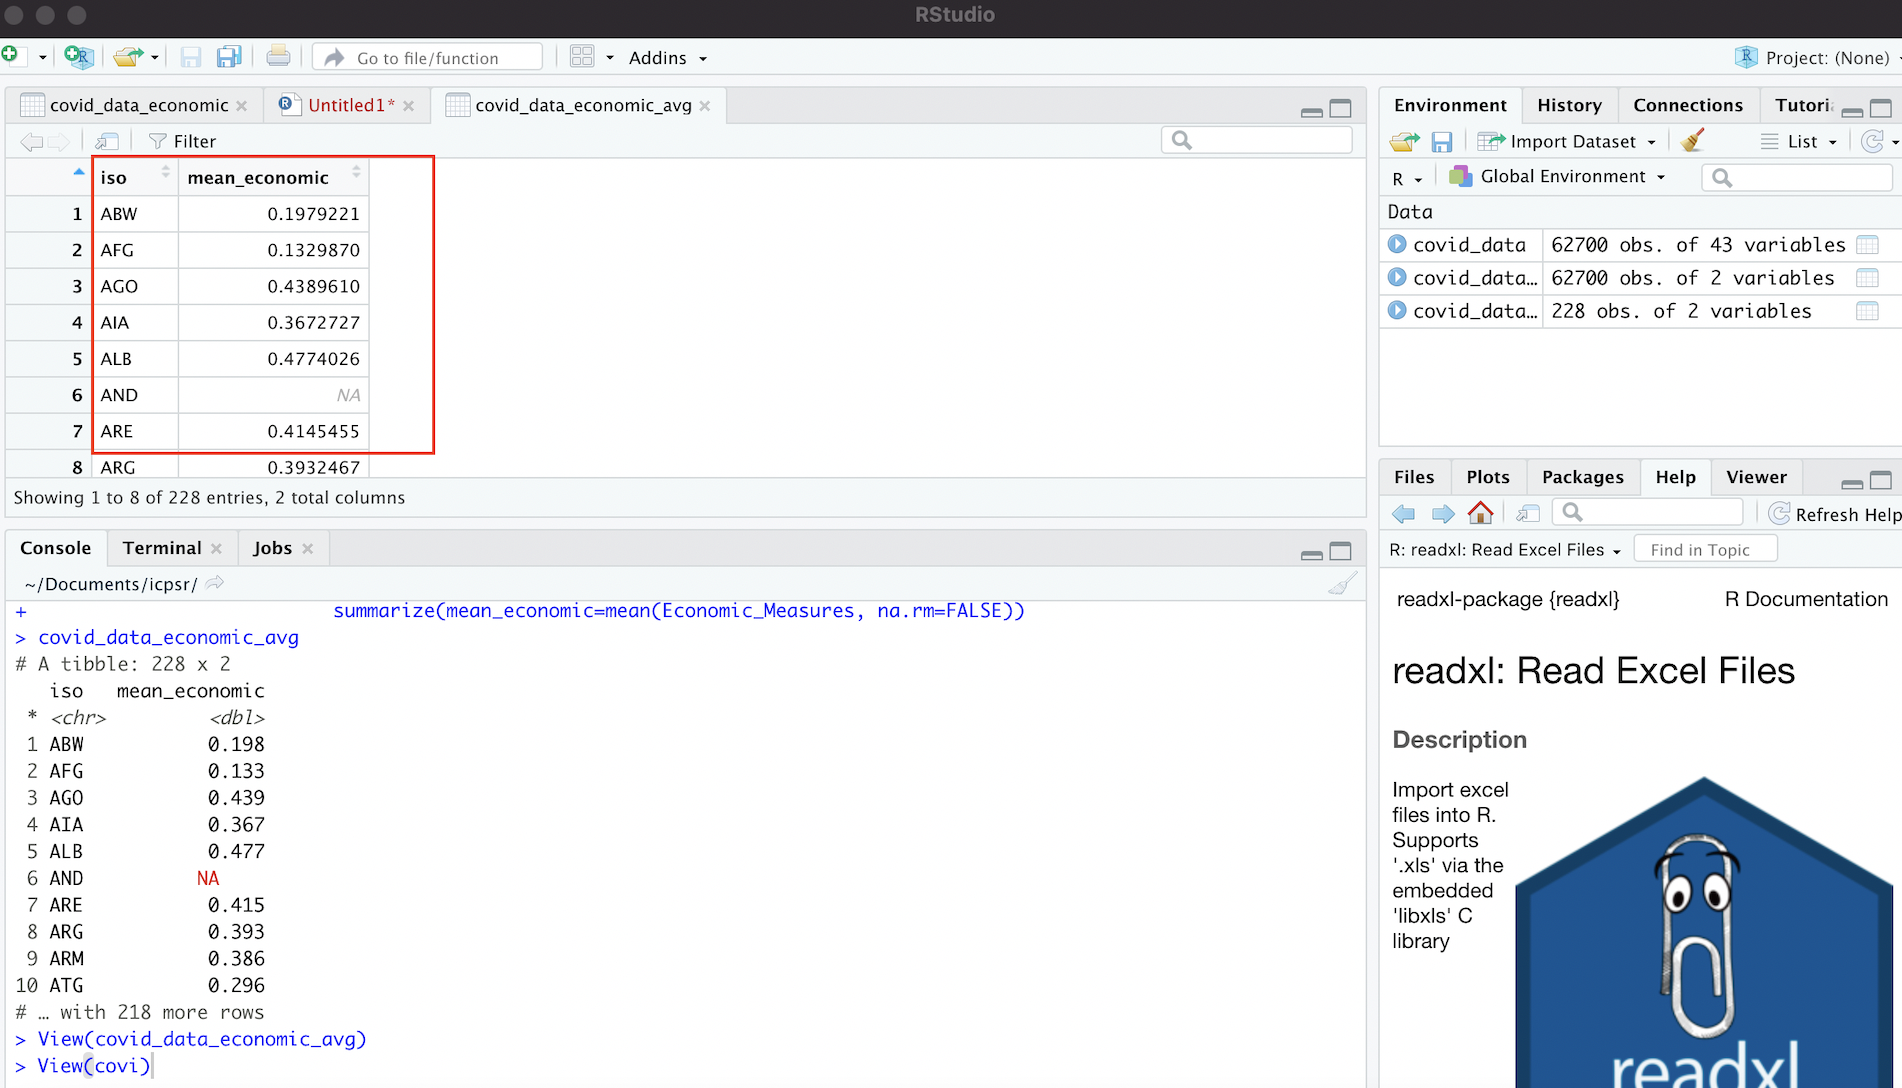
\includegraphics[width=1\linewidth]{images/mean_economic} \textbackslash caption\{Dataset of Country-Level Averages for ``Economic\_Measures'' Index\}\label{fig:unnamed-chunk-37}
\textbackslash end\{figure\}

\hypertarget{calculate-summary-statistics}{%
\subsubsection{Calculate Summary Statistics}\label{calculate-summary-statistics}}

Now that we have a dataset containing the country-level average of the ``Economic\_Measures'' index (which is the data we'd like to map), it can be useful to get a sense of how the data is distributed. We can easily do this by using the \texttt{summary} function, which returns a table of summary statistics for a specified variable. The following code produces summary statistics for the ``mean\_economic'' variable within the dataset that is contained in the ``covid\_data\_economic\_average'' dataset (which is written as \texttt{covid\_data\_economic\$mean\_economic}):

\begin{Shaded}
\begin{Highlighting}[]
\FunctionTok{summary}\NormalTok{(covid\_data\_economic\_avg}\SpecialCharTok{$}\NormalTok{mean\_economic)}
\end{Highlighting}
\end{Shaded}

\begin{verbatim}
##    Min. 1st Qu.  Median    Mean 3rd Qu.    Max.    NA's 
##  0.0000  0.2787  0.3930  0.3853  0.5074  0.7236      30
\end{verbatim}

\hypertarget{join-datasets}{%
\subsection{Join Datasets}\label{join-datasets}}

\begin{Shaded}
\begin{Highlighting}[]
\CommentTok{\# Join dataset with country{-}level means for "Economic\_Measures" index (in "covid\_data\_economic" object) to spatial dataset of world boundaries (in "country\_boundaries" object), based on common 3{-}Digit ISO Codes}
\NormalTok{worldmap\_covid\_data\_economic}\OtherTok{\textless{}{-}}\FunctionTok{full\_join}\NormalTok{(country\_boundaries, covid\_data\_economic\_avg, }\AttributeTok{by=}\FunctionTok{c}\NormalTok{(}\StringTok{"iso\_a3"}\OtherTok{=}\StringTok{"iso"}\NormalTok{))}
\end{Highlighting}
\end{Shaded}

\begin{Shaded}
\begin{Highlighting}[]
\NormalTok{worldmap\_covid\_data\_economic}\OtherTok{\textless{}{-}}\NormalTok{worldmap\_covid\_data\_economic }\SpecialCharTok{\%\textgreater{}\%} \FunctionTok{relocate}\NormalTok{(name, mean\_economic)}
\end{Highlighting}
\end{Shaded}

\hypertarget{make-maps}{%
\subsection{Make Maps}\label{make-maps}}

\begin{Shaded}
\begin{Highlighting}[]
\NormalTok{map1}\OtherTok{\textless{}{-}}\FunctionTok{tm\_shape}\NormalTok{(worldmap\_covid\_data\_economic)}\SpecialCharTok{+}
        \FunctionTok{tm\_polygons}\NormalTok{(}\AttributeTok{col=}\StringTok{"mean\_economic"}\NormalTok{, }\AttributeTok{n=}\DecValTok{8}\NormalTok{, }\AttributeTok{style=}\StringTok{"jenks"}\NormalTok{, }\AttributeTok{palette=}\StringTok{"BuGn"}\NormalTok{)}
\end{Highlighting}
\end{Shaded}

\begin{Shaded}
\begin{Highlighting}[]
\NormalTok{map1}
\end{Highlighting}
\end{Shaded}

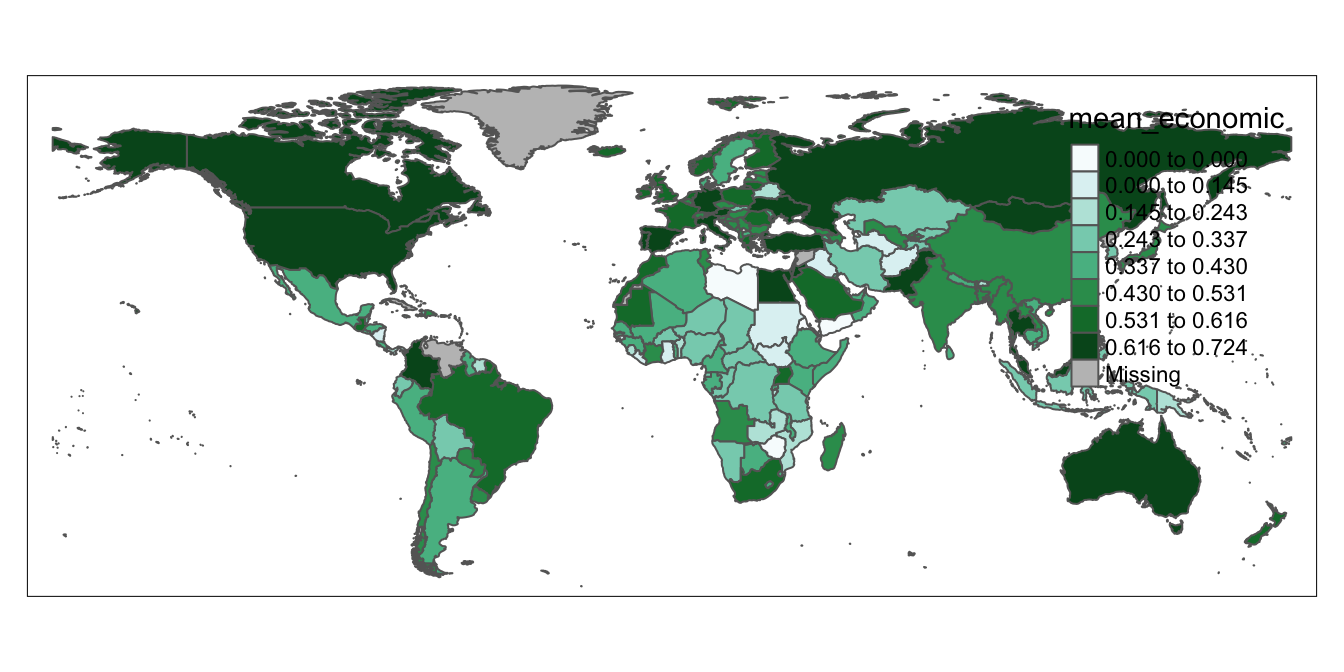
\includegraphics{bookdownproj_files/figure-latex/unnamed-chunk-42-1.pdf}

\end{document}
